\documentclass[11pt]{amsart}
\usepackage{float}
\usepackage{amsfonts, amstext, amsmath, amsthm, amscd, amssymb, upgreek}
\usepackage{bbm}
\usepackage{graphicx, color,  subfigure, wrapfig, overpic}
\usepackage{fullpage}
%\usepackage[all,cmtip]{xy} 
%\usepackage{tikz}
\usepackage{tikz-cd}
%\usepackage{mystyle}

\newcommand{\thmref}[1]{Theorem \ref{#1}}
\newcommand{\prpref}[1]{Proposition \ref{#1}}
\newcommand{\lemref}[1]{Lemma \ref{#1}}
\newcommand{\figref}[1]{Figure \ref{#1}}
\newcommand{\secref}[1]{Section \ref{#1}}
\newcommand{\remref}[1]{Remark \ref{#1}}
\newcommand{\eqnref}[1]{(\ref{#1})}
%\newcommand{\ref}[1]{Figure \ref{#1}}
\newcommand{\comment}[1]{}
\newcommand{\inv}{{-1}} % annoying to type {-1} when taking inverse


\textwidth 6.07in 
\textheight 8.6in 
\oddsidemargin 0.18in
\evensidemargin 0.18in
% \topmargin -0.07in
 
%%  If the following line is uncommented, we see the labels of theorems, figures, etc. in the margins.
% \usepackage[notref,notcite]{showkeys}
\setlength{\marginparwidth}{0.8in}
\let\oldmarginpar\marginpar
\renewcommand\marginpar[1]{\oldmarginpar[\raggedleft\footnotesize #1]%
{\raggedright\footnotesize #1}}

%This command stops the Math Review numbers appearing in the references! 
\AtBeginDocument{
   \def\MR#1{}
}
\newcommand{\Sp}{{\rm{S}}}
\newcommand{\C}{\mathbb{C}}
\newcommand{\R}{\mathbb{R}}
\newcommand{\Q}{\mathbb{Q}}
\newcommand{\Z}{\mathbb{Z}}
\newcommand{\N}{\mathbb{N}}
\newcommand{\CC}{\mathbb{C}}
\newcommand{\RR}{\mathbb{R}}
\newcommand{\HH}{\mathbb{H}}
\newcommand{\ZZ}{\mathbb{Z}}
\newcommand{\bfloor}[1]{\left\lfloor #1\right\rfloor}
\renewcommand{\P}{\mathcal P}
\newcommand{\A}{\mathcal A}
\newcommand{\W}{\mathcal W}
\newcommand{\vol}{{\rm vol}}
\newcommand{\cut}{{\backslash \backslash}}
\newcommand{\bdy}{\partial}
\newcommand{\voct}{{v_{\rm oct}}}
\newcommand{\vtet}{{v_{\rm tet}}}
\renewcommand{\L}{\mathcal L}
\newcommand{\cp}{\mathcal{C}}
\newcommand{\toF}{{\overset{F}{\longrightarrow}}}
\newcommand{\K}{\upkappa}

\def\co{\colon\thinspace}


\newcommand{\torus}{{\mathbb{T}^2}}
\newcommand{\sT}{{\mathcal{T}}}

\newcommand{\RRR}{{\underline{\mathfrak{R}}}}
\newcommand{\QQQ}{{\underline{\mathfrak{Q}}}}
\newcommand{\CCC}{{\underline{\mathfrak{C}}}}
\newcommand{\PPP}{{\underline{\mathbf{\Phi}}}}
\newcommand{\TTT}{{\underline{\mathbf{\Theta}}}}
\newcommand{\LLL}{{\underline{\mathfrak{L}}}}

\newcommand{\cev}[1]{\overset{\leftarrow}{#1}}

\newcommand{\del}{\partial}
\newcommand{\ddd}[1]{{\frac{\del}{\del #1}}}
\newcommand{\vphi}{\varphi}
\newcommand{\veps}{\varepsilon}
\newcommand{\llong}{{\text{long}}}
\newcommand{\Span}{{\text{span}}}
\newcommand{\Pol}{{\text{Pol}}}
\newcommand{\toruscomp}[1]{{\torus \times I - #1}}

\theoremstyle{plain}
\newtheorem{theorem}{Theorem}[section]
\newtheorem{corollary}[theorem]{Corollary}
\newtheorem{lemma}[theorem]{Lemma}
\newtheorem{prop}[theorem]{Proposition}
\newtheorem{claim}[theorem]{Claim}
\newtheorem{conjecture}[theorem]{Conjecture}
\newtheorem{example}[theorem]{Example}

\newtheorem*{namedtheorem}{\theoremname}
\newcommand{\theoremname}{testing}
\newenvironment{named}[1]{\renewcommand{\theoremname}{#1}\begin{namedtheorem}}{\end{namedtheorem}}
\theoremstyle{definition}
\newtheorem{define}[theorem]{Definition}
\newtheorem{definition}[theorem]{Definition}
\newtheorem{question}[theorem]{Question}
\newtheorem{remark}[theorem]{Remark}

\title{Hyperbolicity of Augmented Links in the Thickened Torus}


\author[Alice Kwon and Ying Hong Tham]{Alice Kwon and Ying Hong Tham}


\begin{document}
\maketitle

\begin{abstract}
For a hyperbolic link $K$ in the thickened torus, We show there is a decomposition of the complement
of a link $L$, obtained from augmenting $K$, into torihedra. We further decompose 
the torihedra into angled pyramids and finally angled tetrahedra. These fit into an angled structure 
on a triangulation of the link complement, and thus by \cite{Casson-Rivin}, this shows
that $L$ is hyperbolic.  
\end{abstract}

\section{Introduction}
\label{s:intro}

Given a twist reduced diagram of a link $K$, \emph{augmenting} is a process in
which an unknotted circle component (augmentation) is added to one or more twist
regions (a single crossing or a maximal string of bigons) of $K$. The added circle
component allows us to remove full twists at the twist region of $K$. If the
twist region has an odd number of crossings then all but one crossing is
removed, whereas if the twist region has an even number of crossings then all
are removed. We can remove full twists by a standard argument using a Dehn twist 
on the complement of the crossing circle. The newly obtained link is called an 
\emph{augmented link} and the newly obtained diagram is called an 
\emph{augmented link diagram}. See Figure
\ref{fig:Augmentations}. 

Adams showed in \cite{CA} that given a hyperbolic alternating link $K$ in
$\Sp^3$ the link $L$ obtained by augmenting $K$ is hyperbolic. In this paper we
investigate if this statement holds for links in the thickened torus i.e. if $L$
is a link obtained from augmenting a hyperbolic alternating link $K$ in the
thickened torus. We define augmenting similarly for links in the thickened torus
with their associated link diagram on $\torus \times \{0\}.$ 

Menasco \cite{Menasco} showed there are decompositions of the complements of
alternating links in $\Sp^3$ into two topological polyhedra, a top polyhedron and a bottom
polyhedron.  For alternating links $K$ in the thickened torus, Champanerkar,
Kofman and Purcell \cite{CKP2} showed that there is a decomposition of the
complement of $K$ into objects called torihedra, which we think of as
counterparts to Menasco's decomposition of links in $\Sp^3$ into polyhedra, for
links in the thickened torus. Just like Menasco's decomposition, one obtains a
top and a bottom torihedron.


In \secref{s:auglinks} we show that for augmented
links in the thickened torus one can also obtain a decomposition of the
complement into a top and bottom torihedron.  In \secref{s:hyperbolicity}, we
prove that many augmented alternating links in the thickened torus are
hyperbolic.


We point out that \cite{kwon2020fully}, the first author
proved that \emph{fully} augmented links in the thickened torus
are hyperbolic, so this paper can be seen as a generalization
of that work.


While revising this paper,
we learned that \cite{adams2021generalized}
proves a generalization of our work here,
showing hyperbolicity of generalized augmented links
in an arbitrary thickened surface.
We note that our approach, based on angle structures,
is different from theirs, which is based on topological arguments.



 \begin{figure}
 \centering  
 \begin{tabular}{cc}
 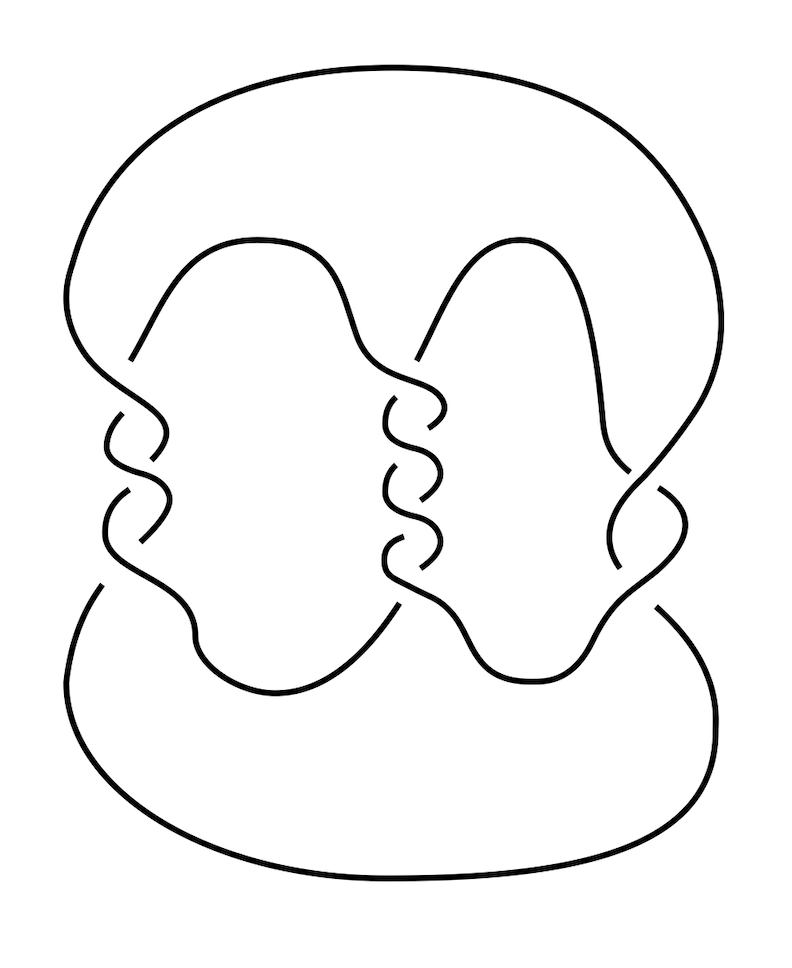
\includegraphics [height=4cm]{augmentation1.png}&
  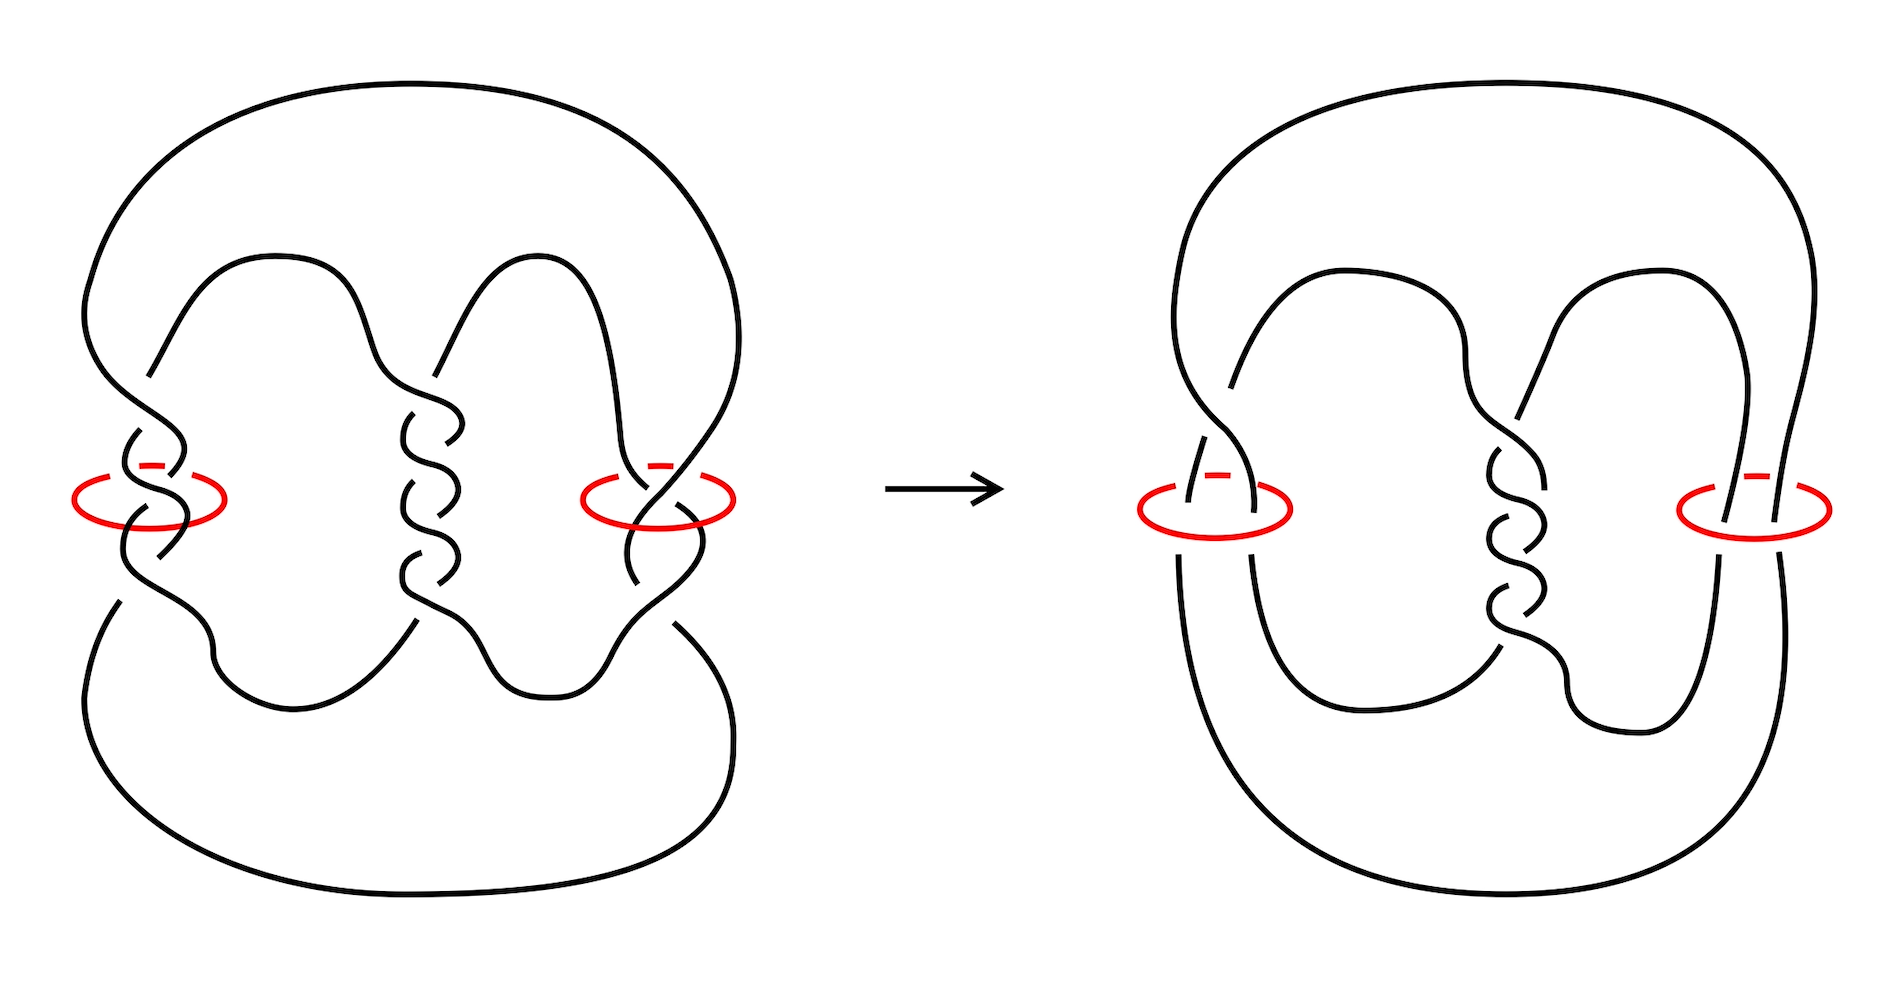
\includegraphics [height=4cm]{augmentation2.png}\\
  (a)&(b)
  \end{tabular}
 \caption{The left shows a pretzel knot before augmentation and the right shows after augmentation}
 \label{fig:augmentationS3}
 \end{figure}
 
 
 %%%%%%%%%%%%%%%%%%%%%%%%%%%%%%%%%%%%%%%%%%%%%%%%%%%%%%%% 
\section{Augmented Links}
\label{s:auglinks}

Champanerkar, Kofman and Purcell have studied alternating links in the thickened torus \cite{CKP2}. They define a link in the thickened torus as a quotient of a biperiodic alternating link as follows,
 
\begin{define}
\label{def:biperiodiclink}
A \emph{biperiodic alternating link} $\mathcal{L}$ is an infinite link
which has a projection onto
$\R^2$ which is invariant under an action of a two dimensional lattice $\Lambda$
by translations, such that $L=\mathcal{L}/\Lambda$ is an alternating link in
$\torus \times I$, where $I = (-1,1)$, with the projection on $\torus \times \{0\}$.   
\end{define}

\begin{remark}
Since $\torus \times I \cong \Sp^3 - H$, where $H$ is a Hopf link. The complement $\torus \times I- L = \Sp^3 - (L \cup H)$.
\end{remark}

Champanerkar, Kofman and Purcell \cite{CKP2} extended the definition of prime links in $\Sp^3$ for links in $\torus \times I$ called weakly prime. 

 \begin{define} \label{def:weaklyprime}
	 A diagram of a link $L$ is \emph{weakly prime} if whenever a disk is embedded in the diagram surface meets the diagram transversely in exactly two edges, then the disk contains a simple edge of the diagram and no crossings.
\end{define}


\begin{define}
A \emph{twist region} in a link diagram of $L=\mathcal{L}/\Lambda$ in $\torus
\times I$, is the quotient of a twist region in the biperiodic link
$\mathcal{L}$. 
%a string of bigons, or a single crossing in the diagram on the universal cover of $\torus \times I$ is called a .  
A biperiodic link
$\mathcal{L}$ is called \emph{twist-reduced} if for any simple closed curve on
the plane that intersects the diagram of $\mathcal{L}$ transversely in four points, with two
points adjacent to one crossing and the other two points adjacent to another
crossing, the simple closed curve bounds a subdiagram consisting of a (possibly
empty) collection of bigons strung end to end between these crossings. We say
the diagram of $L$ is \emph{twist-reduced} if it is the quotient of a twist-reduced biperiodic
link diagram.  \end{define}

Now we can define augmentation for a link in $\torus \times I$ the same way we
define augmentation for links in $\Sp^3$. For a link in $\torus \times I$, the
crossing circles are added to the diagram projected onto $\torus \times \{0\}$.
Let $D(L)$ be a twist reduced diagram of a link $L$ in $\torus \times I$, we define
\emph{augmenting} as a process in which an unknotted circle component is added
to one or more twist regions of $D(L)$. See Figure \ref{fig:Augmentations}

\begin{remark}
If $L$ is augmented at \emph{every} crossing/twist site we say $L$ is \emph{fully} augmented.
\end{remark}

\begin{figure}
\centering
\begin{tabular}{cccc}
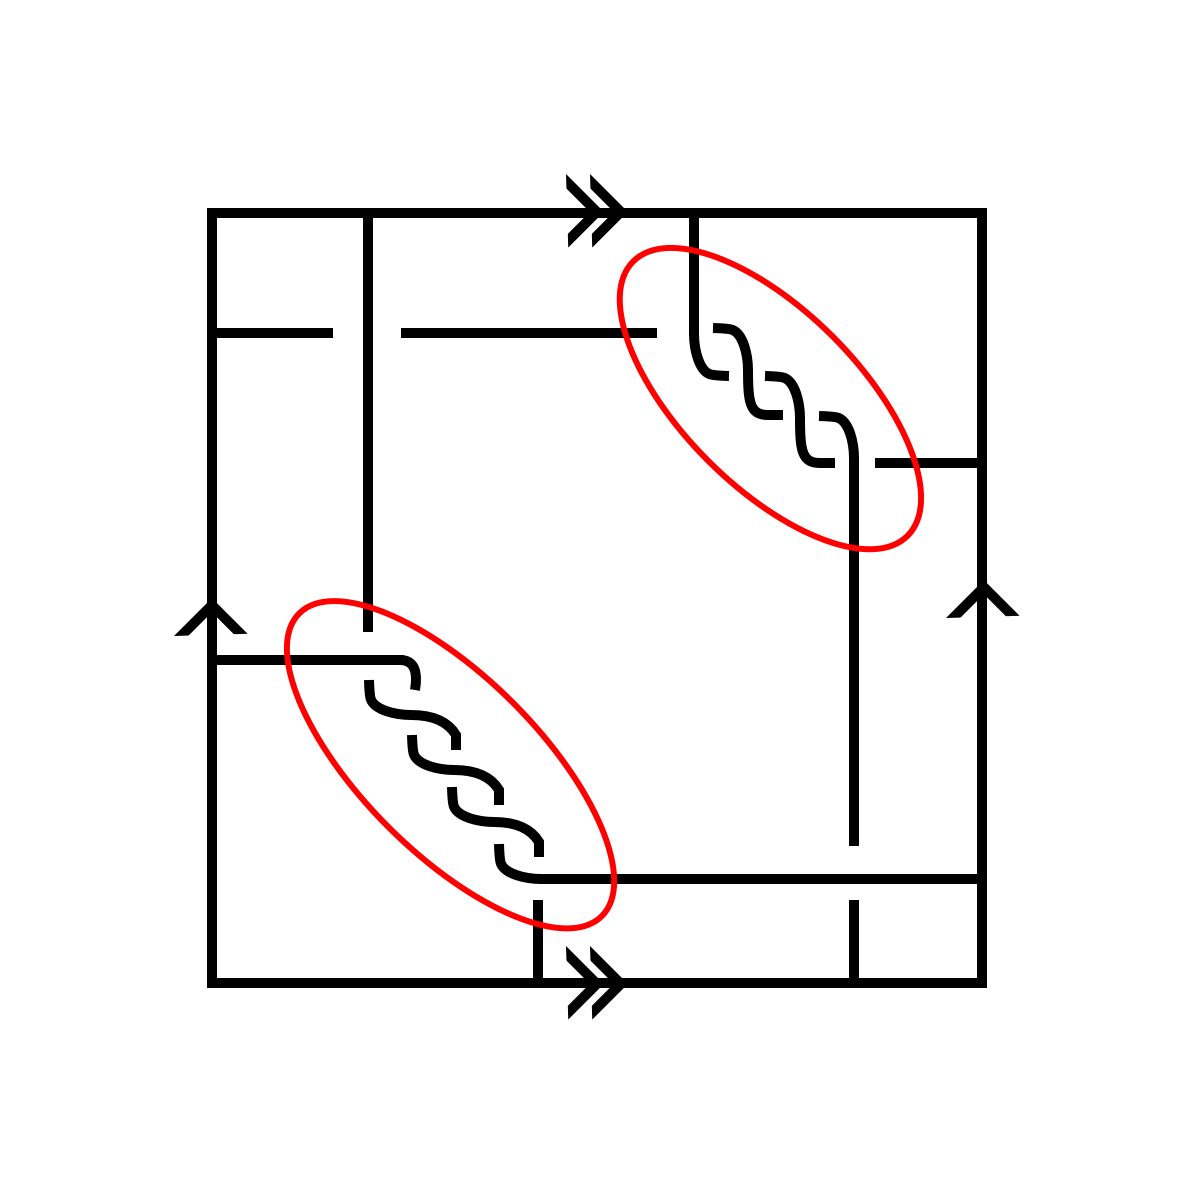
\includegraphics[width=3cm]{fig1.png}&
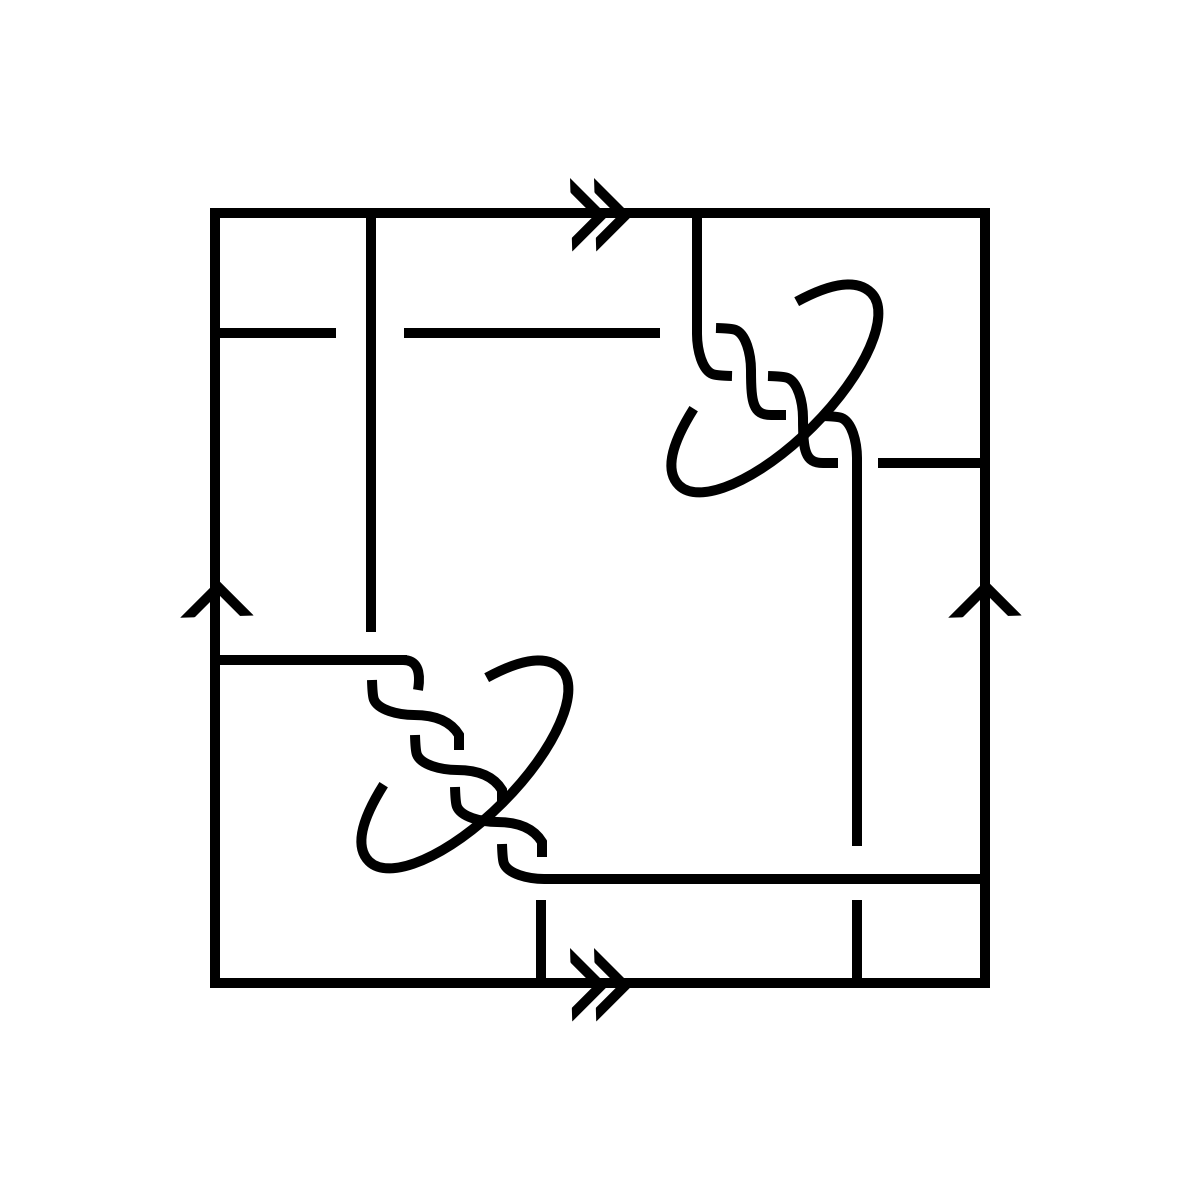
\includegraphics[width=3cm]{twist-augment.png}&
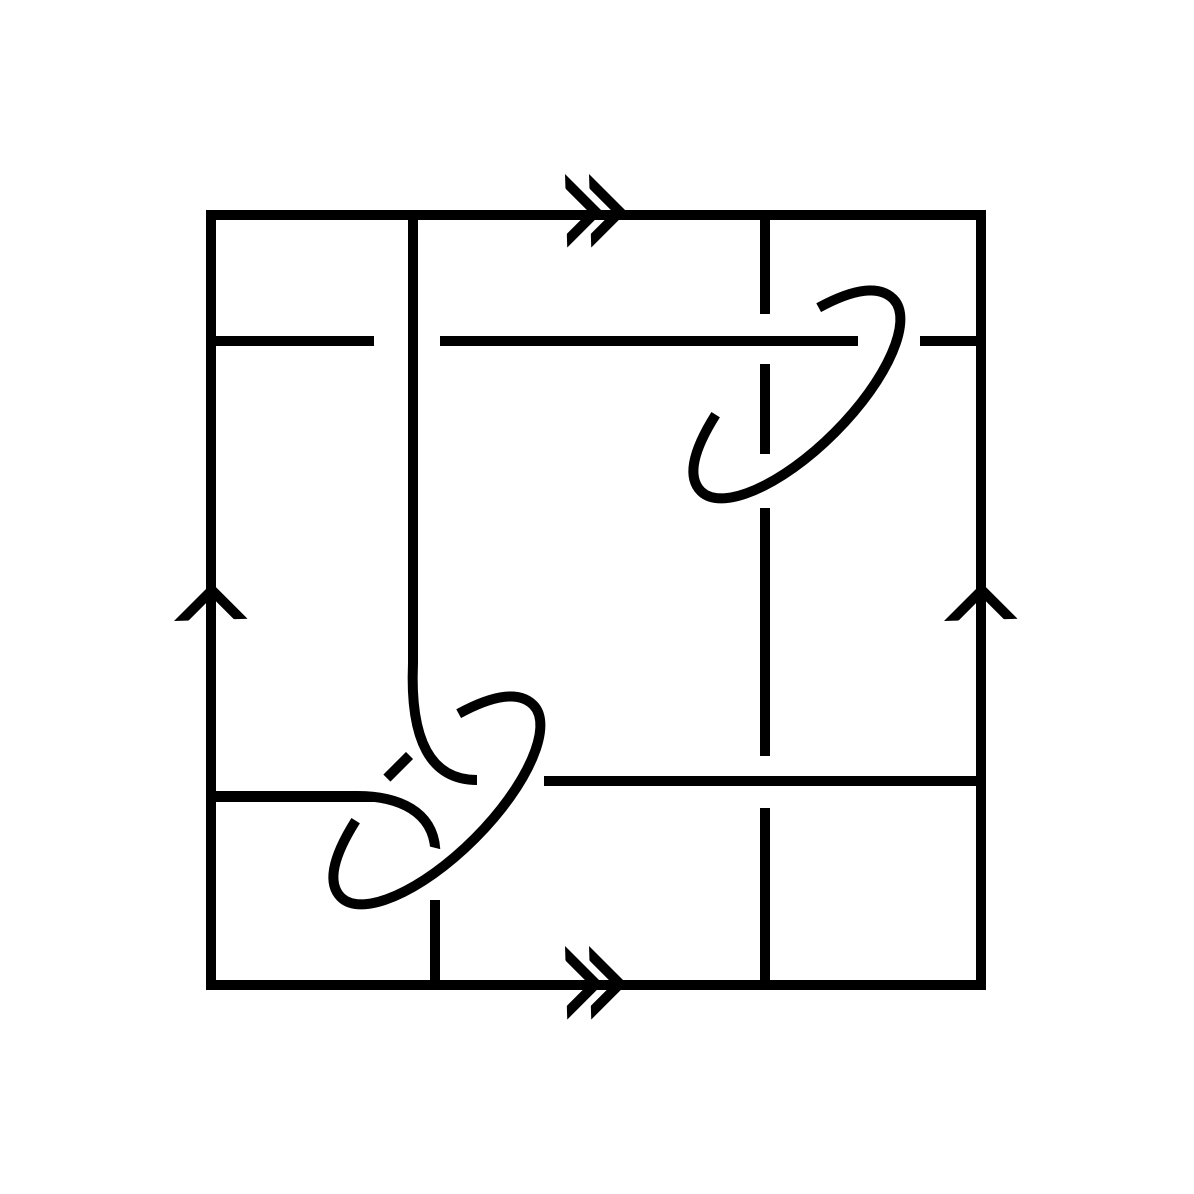
\includegraphics[width=3cm]{fig-2.png}\\
 % 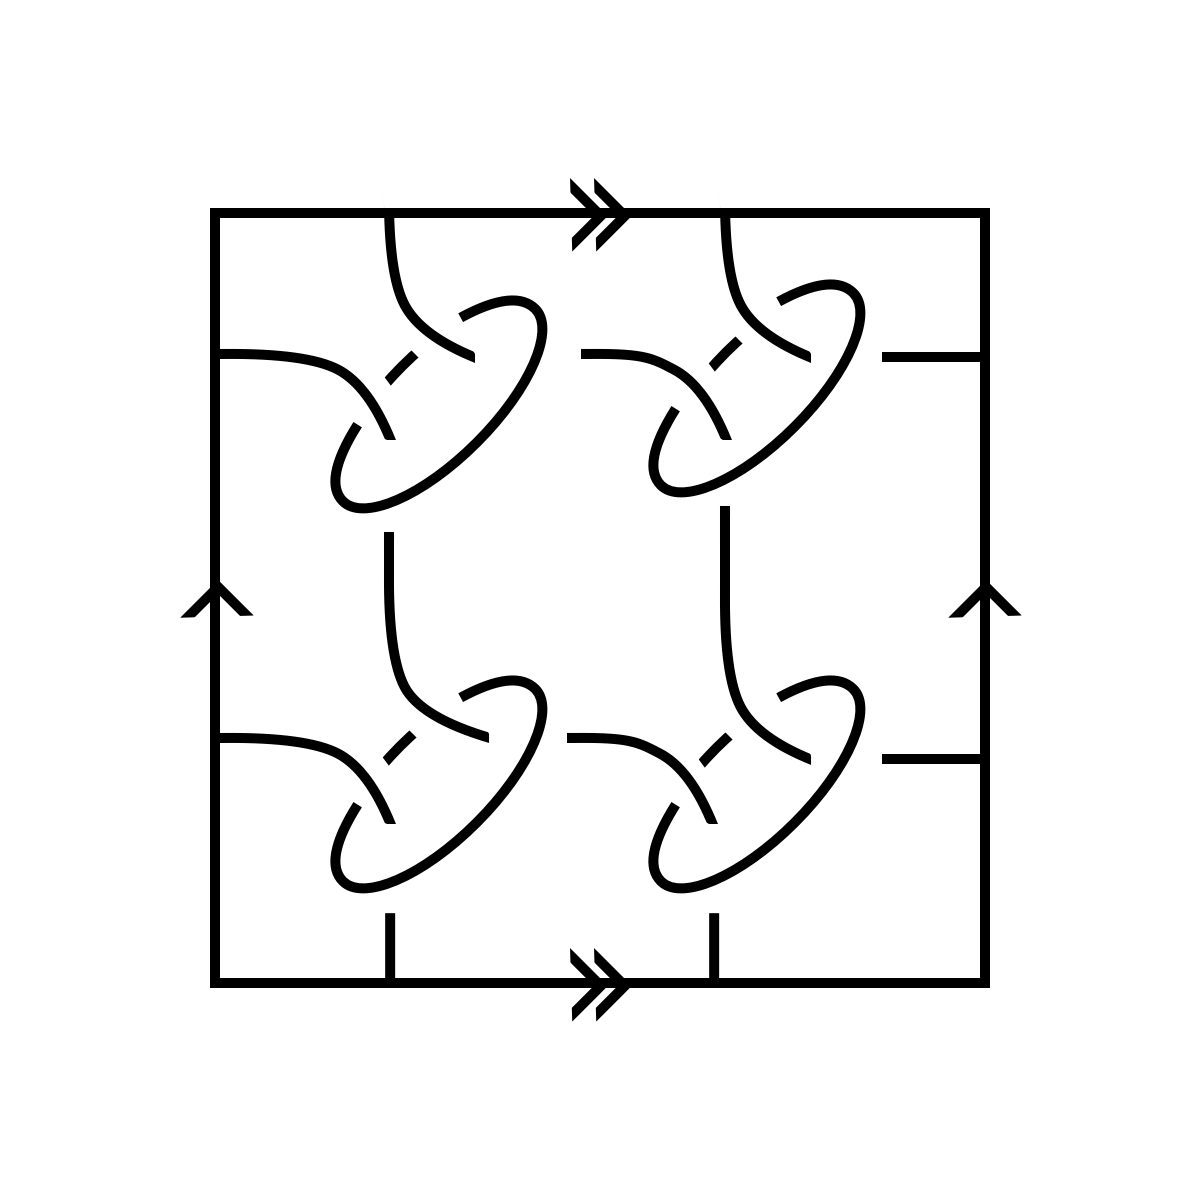
\includegraphics [width=3cm]{fal}\\
A&B&C
\end{tabular}
	 \caption{A: The top right has an odd number of twists while the bottom left has
	 an even number of twists. B: The picture of the link on the right after
	 augmentation twist regions circled in red. C: The link with full twists
	 removed.}
\label{fig:Augmentations}
\end{figure}
%%%%%%%%%%%%%%%%%%%%%%%%%%%%%%%%%%%%%%%%%%%%%%%%%%%% 

\subsection{Torihedral Decomposition of Augmented Alternating Links in Thickened Torus}


We present a method of decomposing an augmented link (not necessarily fully augmented) 
in the thickened torus into
objects called ``torihedra'' as defined below.  Decomposing alternating links in the thickened torus into 
torihedra were first described in \cite{CKP2} then later used for fully augmented links in 
the thickened torus in \cite{kwon2020fully}.
The idea is to combine methods of Menasco
\cite{Menasco} and the use of crossing edges between each crossing of our link
and Lackenby's ``cut-slice-flatten" method \cite{lackenby} on the augmentation
sites.



\begin{define}\cite{CKP2}
\label{def:torihedron}
A \emph{torihedron} $\sT$ is a cone on the torus, 
i.e. $\torus \times [0,1]/(\torus \times \{1\})$, with a cellular graph
$G = G(\sT)$ on $\torus \times \{0\}$.
The \emph{ideal torihedron} $\sT^\circ$ is $\sT$ with the
vertices of $G$ and the vertex $\torus \times \{1\}$ removed. Hence, an ideal
torihedron is homeomorphic to $\torus \times [0,1)$ with a finite set of points
(ideal vertices) removed from $\torus \times \{0\}$.
We refer to the vertex $\torus \times \{1\}$ as the cone point.
\end{define}


For visualization purposes, we typically draw the graph $G(\sT)$ of a
torihedron from the perspective of the cone point $\torus \times \{1\}$.

If the faces of $G(\sT)$ are disks,
then $\sT$ can be decomposed into a union of pyramids,
obtained by coning each face to the cone point of $\sT$.
This also gives a decomposition of the corresponding ideal torihedron
$\sT^\circ$ into ideal pyramids.
We call these the \emph{pyramidal decompositions} of $\sT$ and $\sT^\circ$.

\begin{prop}\label{p:tori_decomp}
Let $L$ be an augmented link in $\torus \times I$.
%Let $G(L)$ be a diagram of the link on $\torus \times \{0\}$.
There is a decomposition of the complement,
$(\torus \times I) - L$ into two ideal torihedra.
\end{prop}

\begin{proof}
We will begin by assuming that there are no half twists. 
Arrange the link diagram of $L$ in the following way: first place the added
circle components perpendicular to the projection plane, $\torus
\times \{0\}$ leaving the remaining part of the link parallel to the projection
plane.  We now place a crossing edge on each crossing of the link so that for
each crossing edge, one end of the edge lies on a bottom strand while the other
end lies on a top strand as in Figure \ref{fig:crossingArc} left.

\begin{figure} 
\centering 
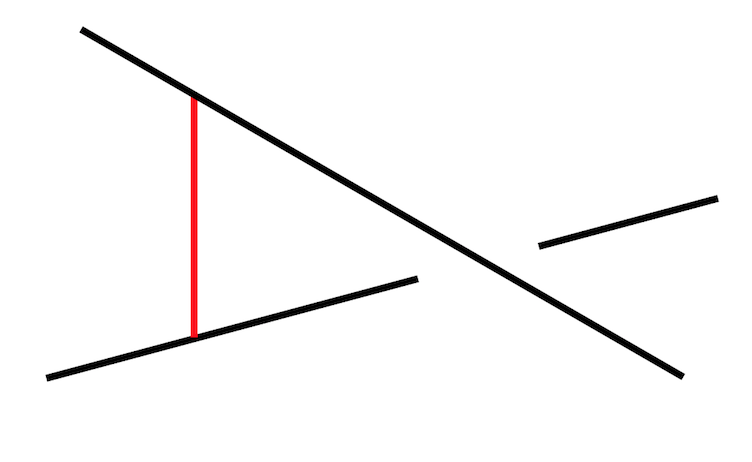
\includegraphics[width=4cm]{crossingArc.png}
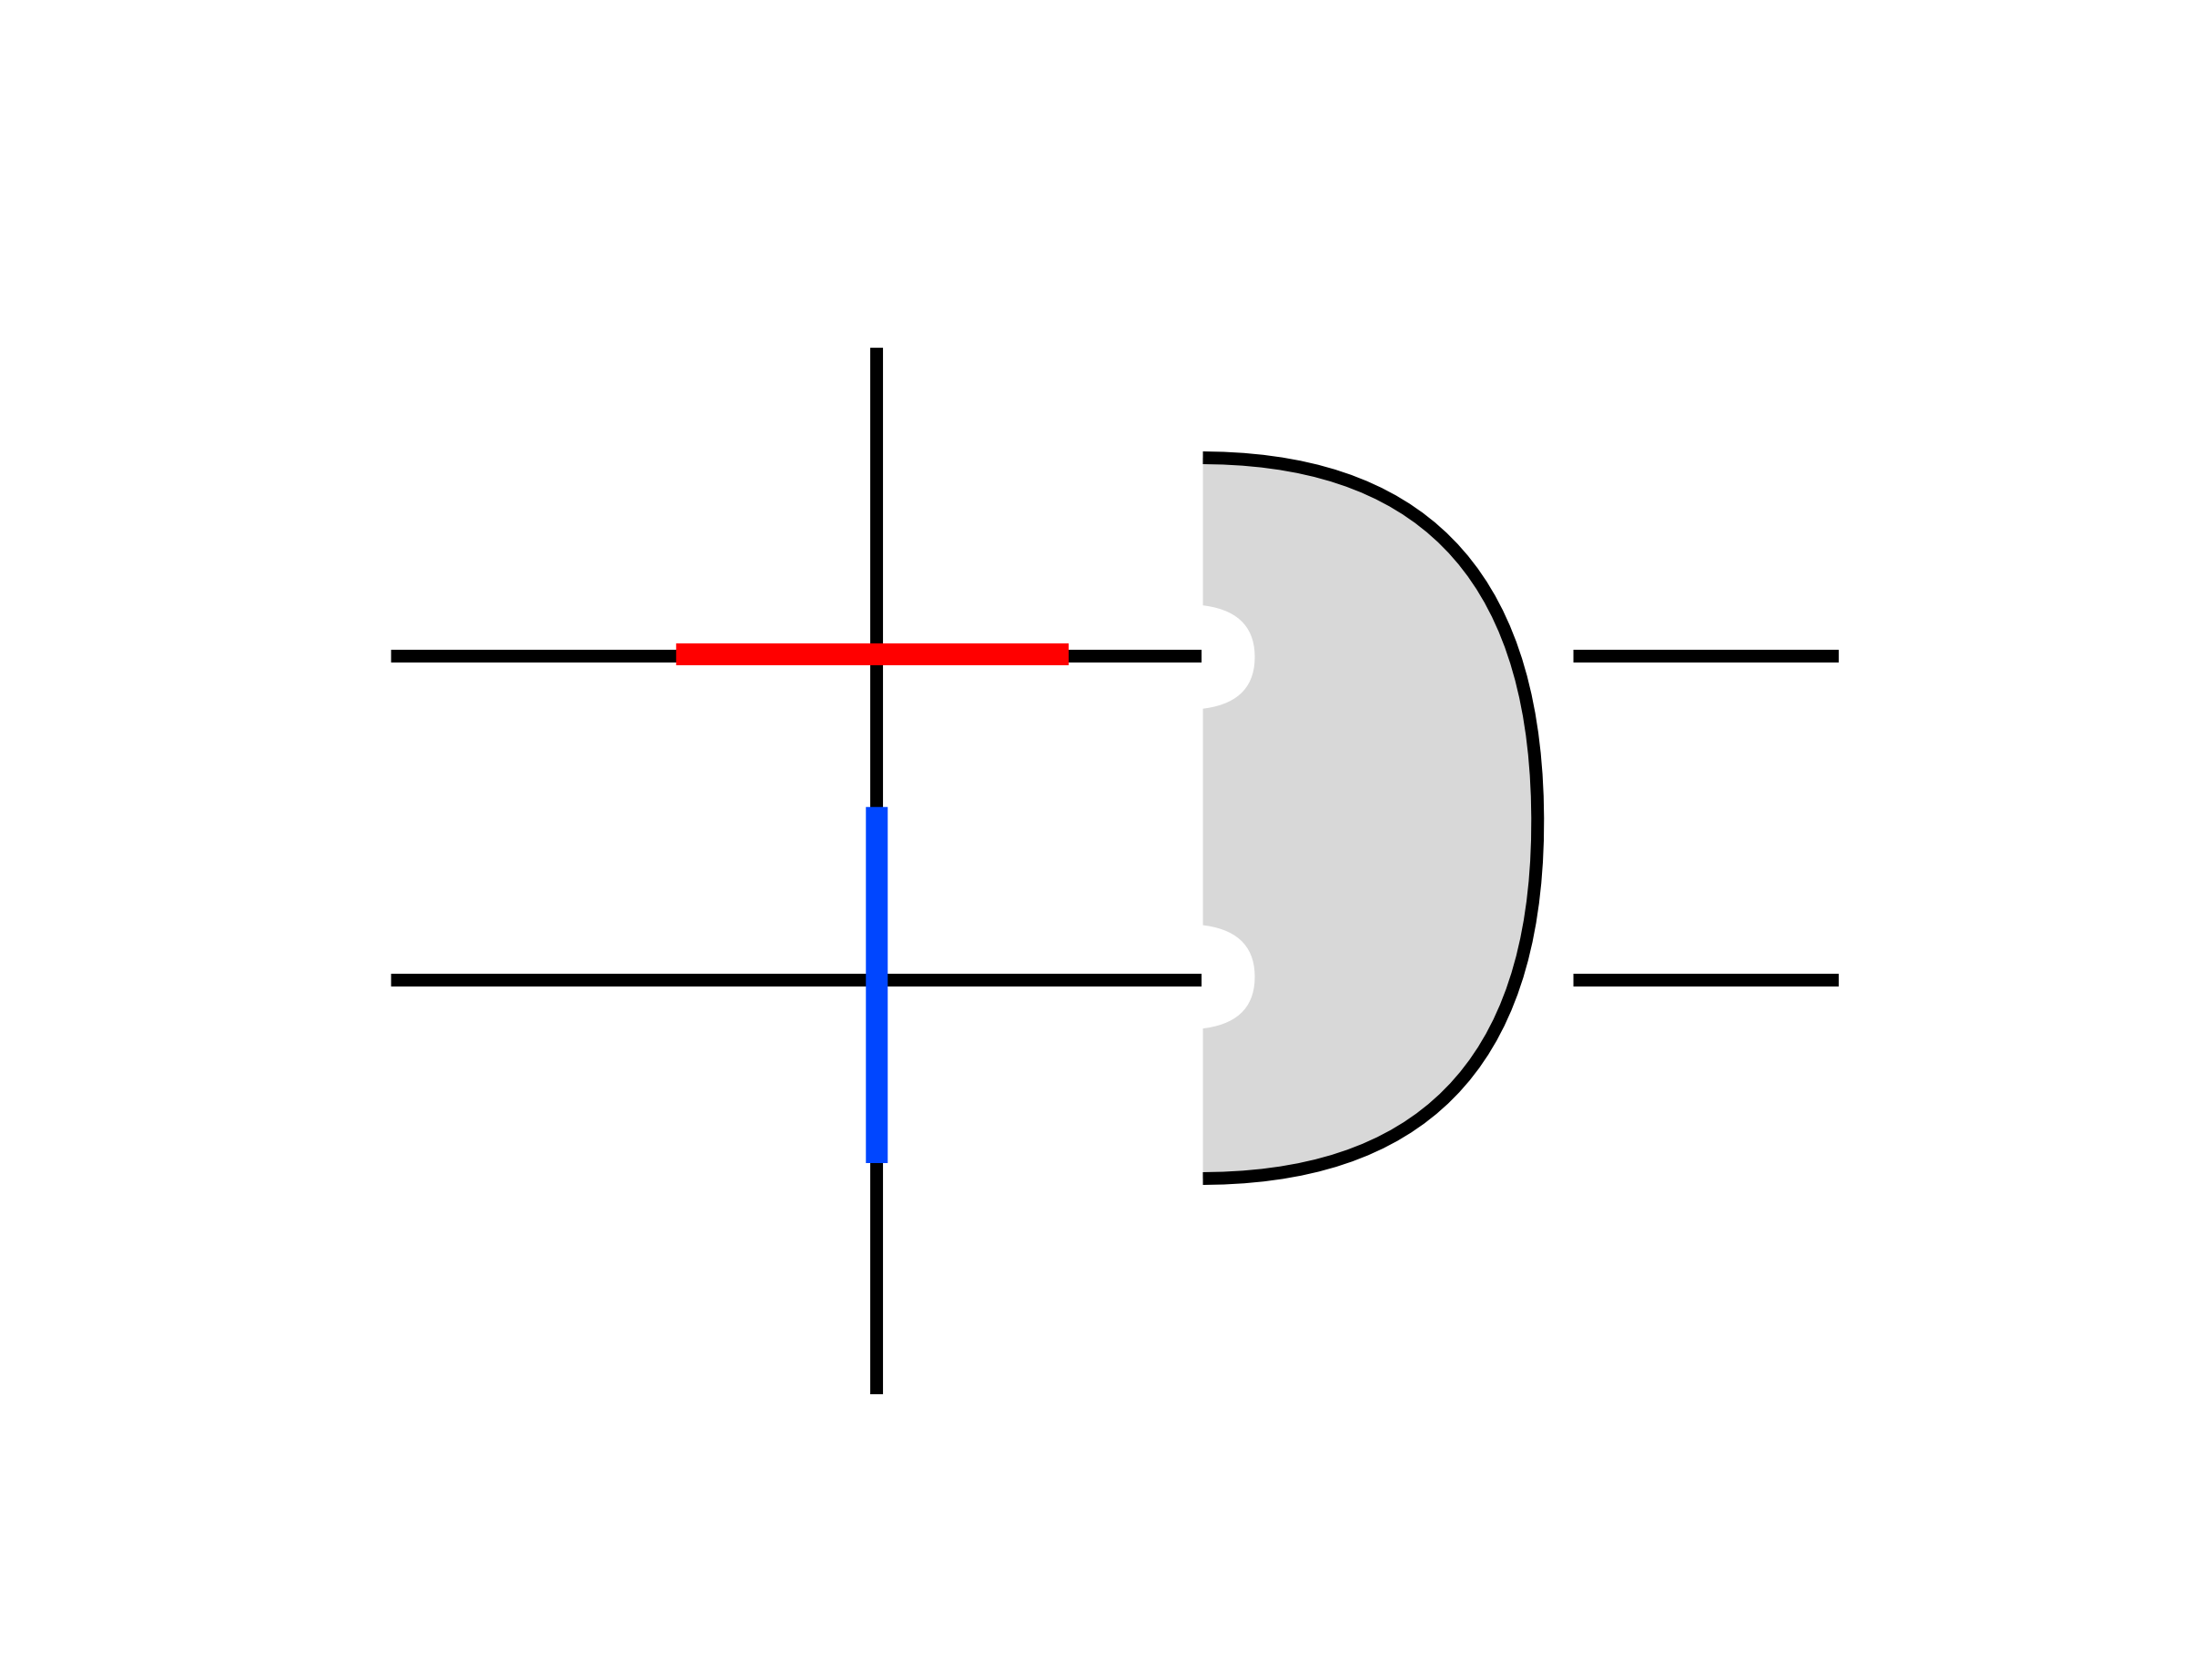
\includegraphics[width=5cm]{crossingPush.png}
\caption{Left: The black strands are
part of the link and the red strand is the crossing edge. Right: The blue and
red edges represent the split crossing edges and the shaded half disk is bounded
by the crossing circle} 
\label{fig:crossingArc} 
\end{figure}

\indent We view the link from the point at infinity from the top. We will push
the top strand to the bottom strand, splitting the crossing edge into two
identical edges as in Figure \ref{fig:crossingArc} right. We push the link
components to infinity and stretch the crossing edge so that we have flattened
the link onto $\torus \times \{0\}$ except for the crossing circles which will
remain perpendicular to the projection plane. 
 
\indent Now place a disk on each crossing circle, so that the disk is bounded by
the crossing circle. We can then cut $\torus \times I$ along $\torus \times \{0\}$ and
focus on the top half, $\torus \times [0,1)$. We will follow the same method on the
bottom half to obtain the second identical torihedron. The disk we place on each
crossing circle is now cut in half. This half disk is now bounded by the
projection plane and the semi-cricle arc of the crossing circle. We push down on
the crossing circle and split the disk into two identical disks. We then push
the arc of each crossing circle to infinity, collapsing them to ideal vertices.
We obtain two triangular faces which represent the disk which look like a
bow-tie as in Figure \ref{fig:falGluings}. 

\begin{figure}
 \centering
 \begin{tabular}{cc}
 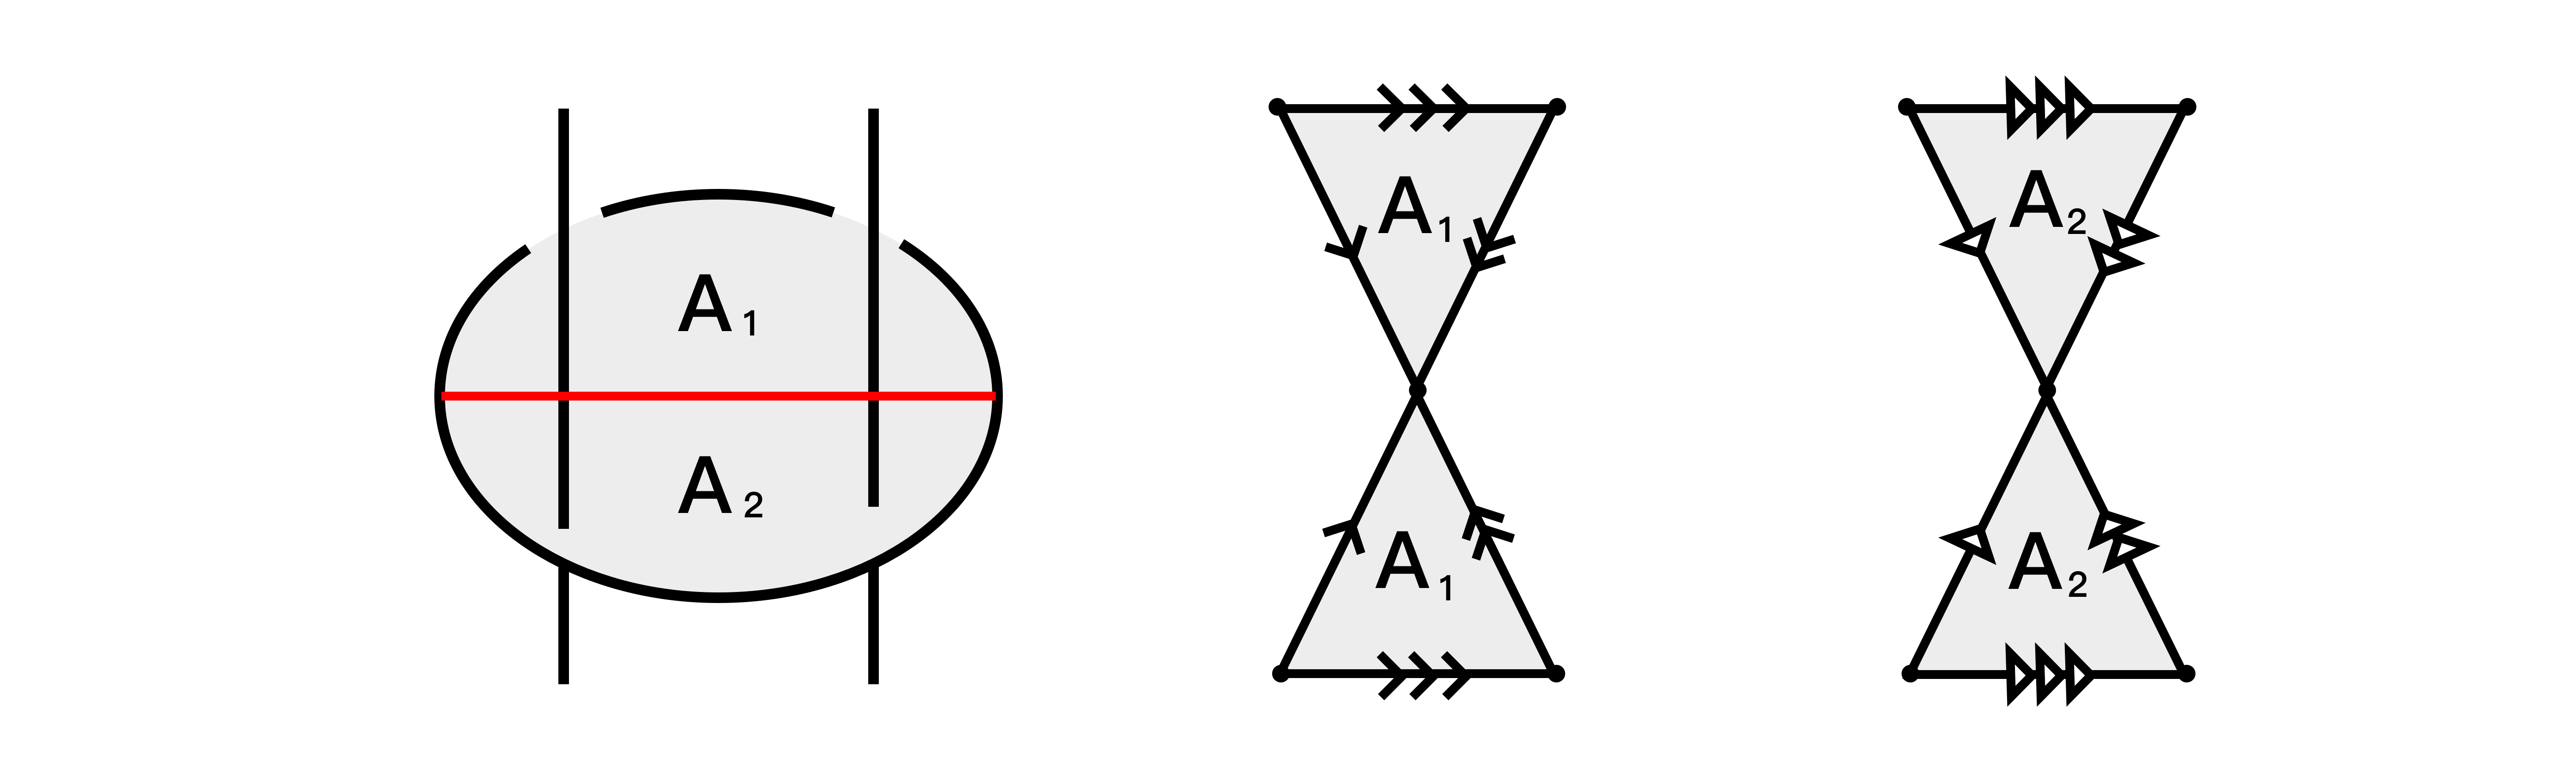
\includegraphics [width=8cm]{falGluing1.png}&
 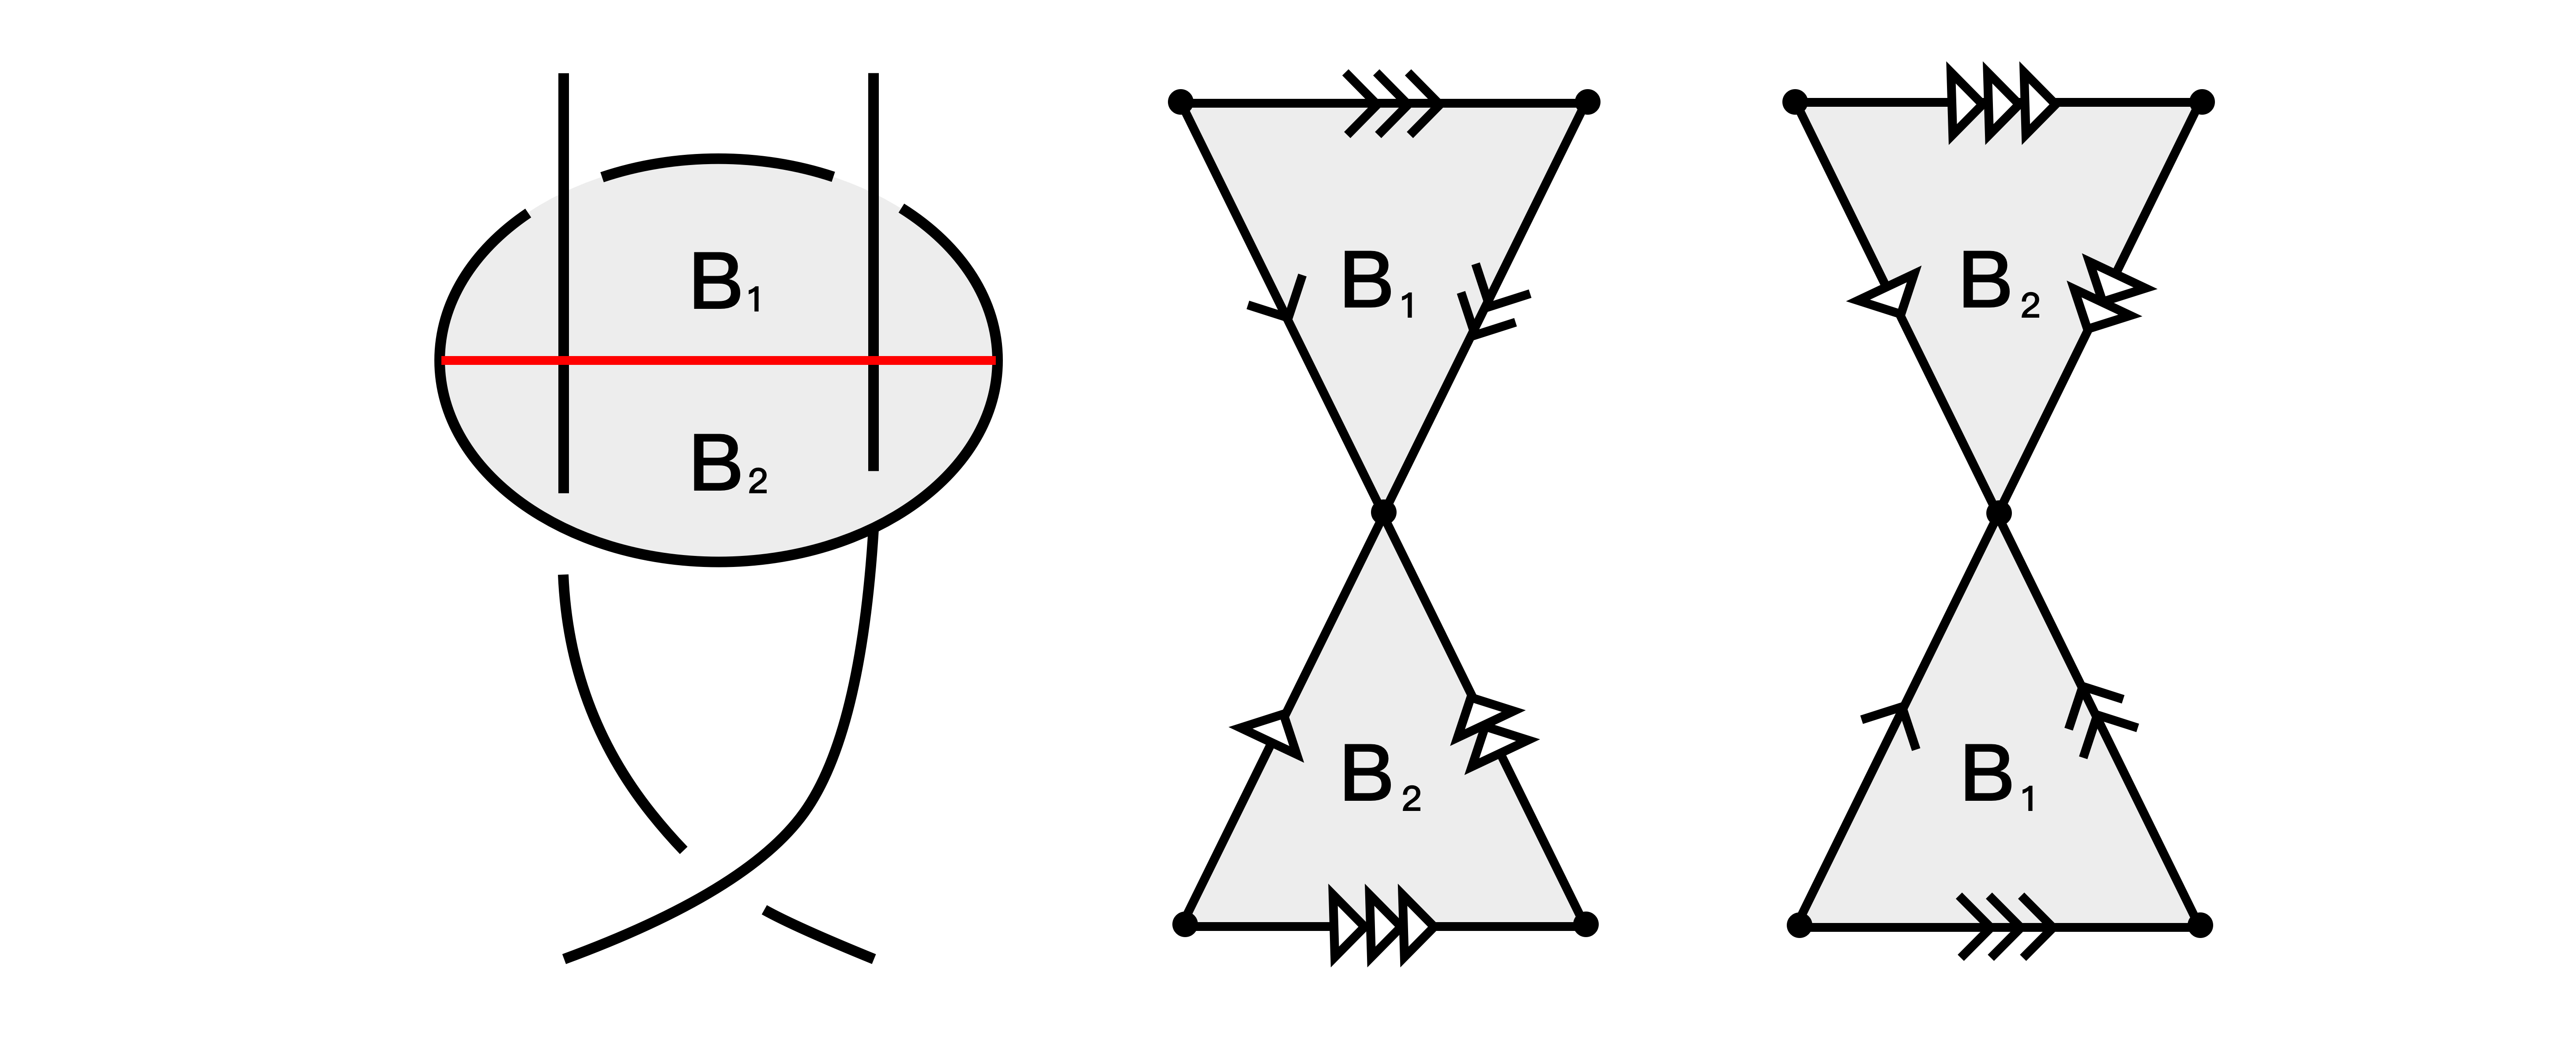
\includegraphics [width=7cm]{falGluing2.png}\\
 (a)&(b)
 \end{tabular}
	\caption{(a) Gluing of bow-ties without half-twists
	(b) Gluing with half-twists}
 \label{fig:falGluings}
 \end{figure}

\indent We repeat the steps for the bottom half of $\torus \times I$, $\torus \times
(-1,0]$. Then we get two torihedra. The graph of each will come from
crossing edges and edges of the disk. Now, if there are half twists we will
decompose the complement of the link the same way as if there are no half twists
and we will identify the two bow-ties as in Figure \ref{fig:falGluings}.
Finally,
we obtain the complement of the link by gluing the two torihedra with the gluing
information given by identifying crossing edges and triangles of the bow-tie. We
glue the faces of the torihedra which do not correspond to a bow-tie with a
$2\pi/n$ twist where $n$ is the number of sides of each face as in Figure
\ref{fig:top-bottom} clockwise or counterclockwise.


For future reference, we will denote the graph for the top and bottom
torihedra by $\Gamma_T(L)$ and $\Gamma_B(L)$, respectively,
where both graphs are viewed from the cone point of the top torihedron
$\torus \times \{1\}$.
Note that if $L = K$ is the non-augmented link,
$\Gamma_T(L)$ is simply the link projection $K$,
and in fact $\Gamma_T(K) = \Gamma_B(K)$.

\end{proof}



%%%%%%%%%%%%%%%%%%%%%%%%%%%%
The Figures \ref{fig:step_one} to \ref{fig:top-bottom} is an example which decomposes the link (C) of Figure
\ref{fig:Augmentations}. 


\begin{figure}[h] 
\centering
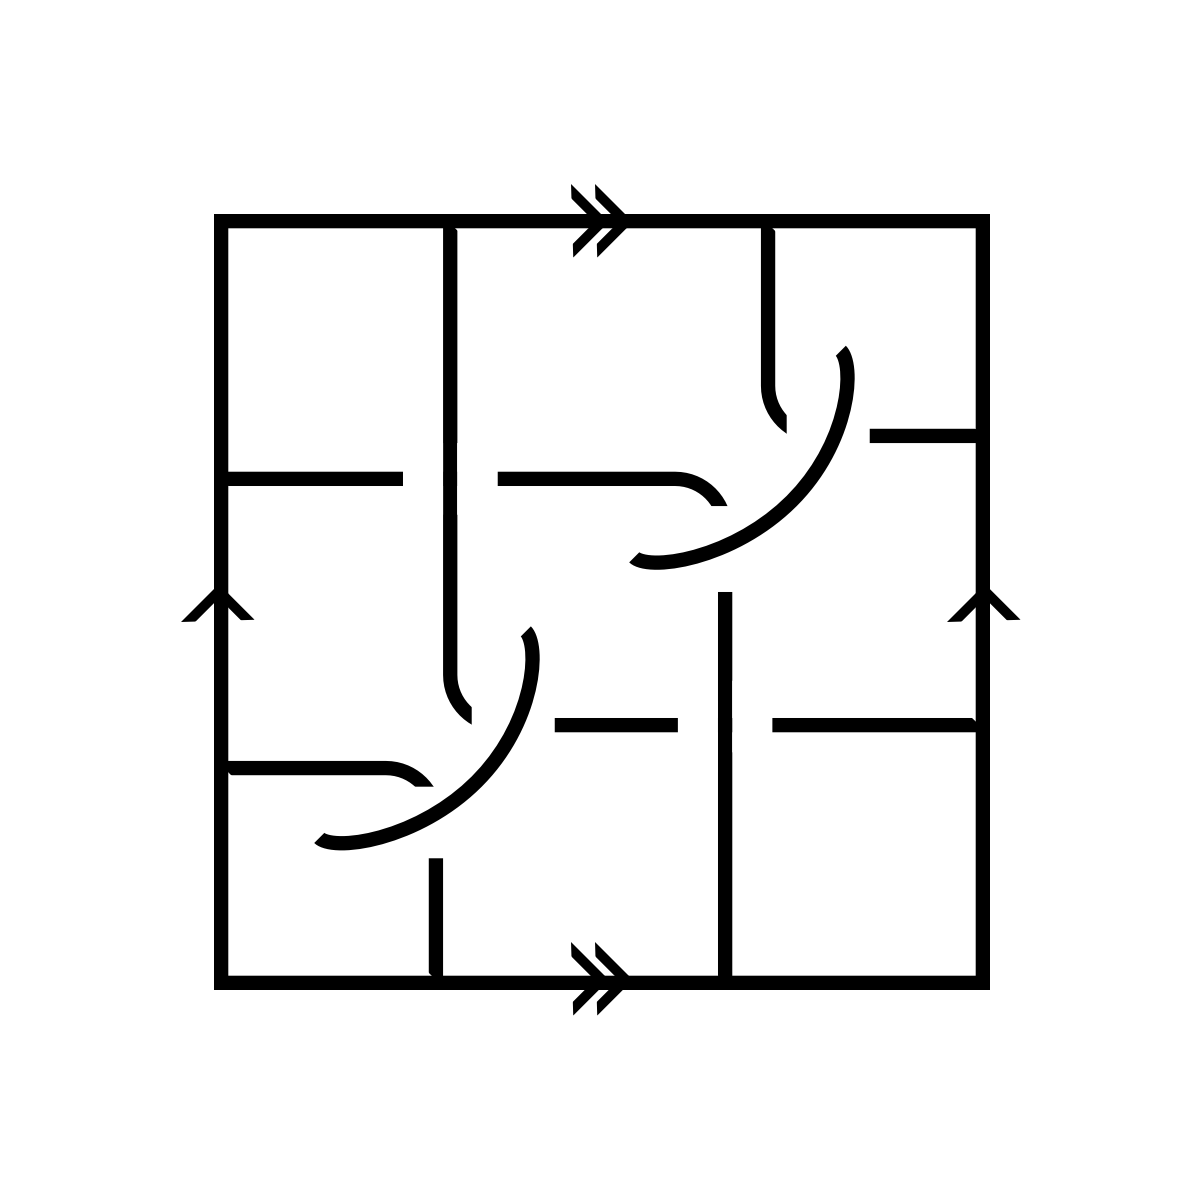
\includegraphics[height=3cm]{fig-3.png}
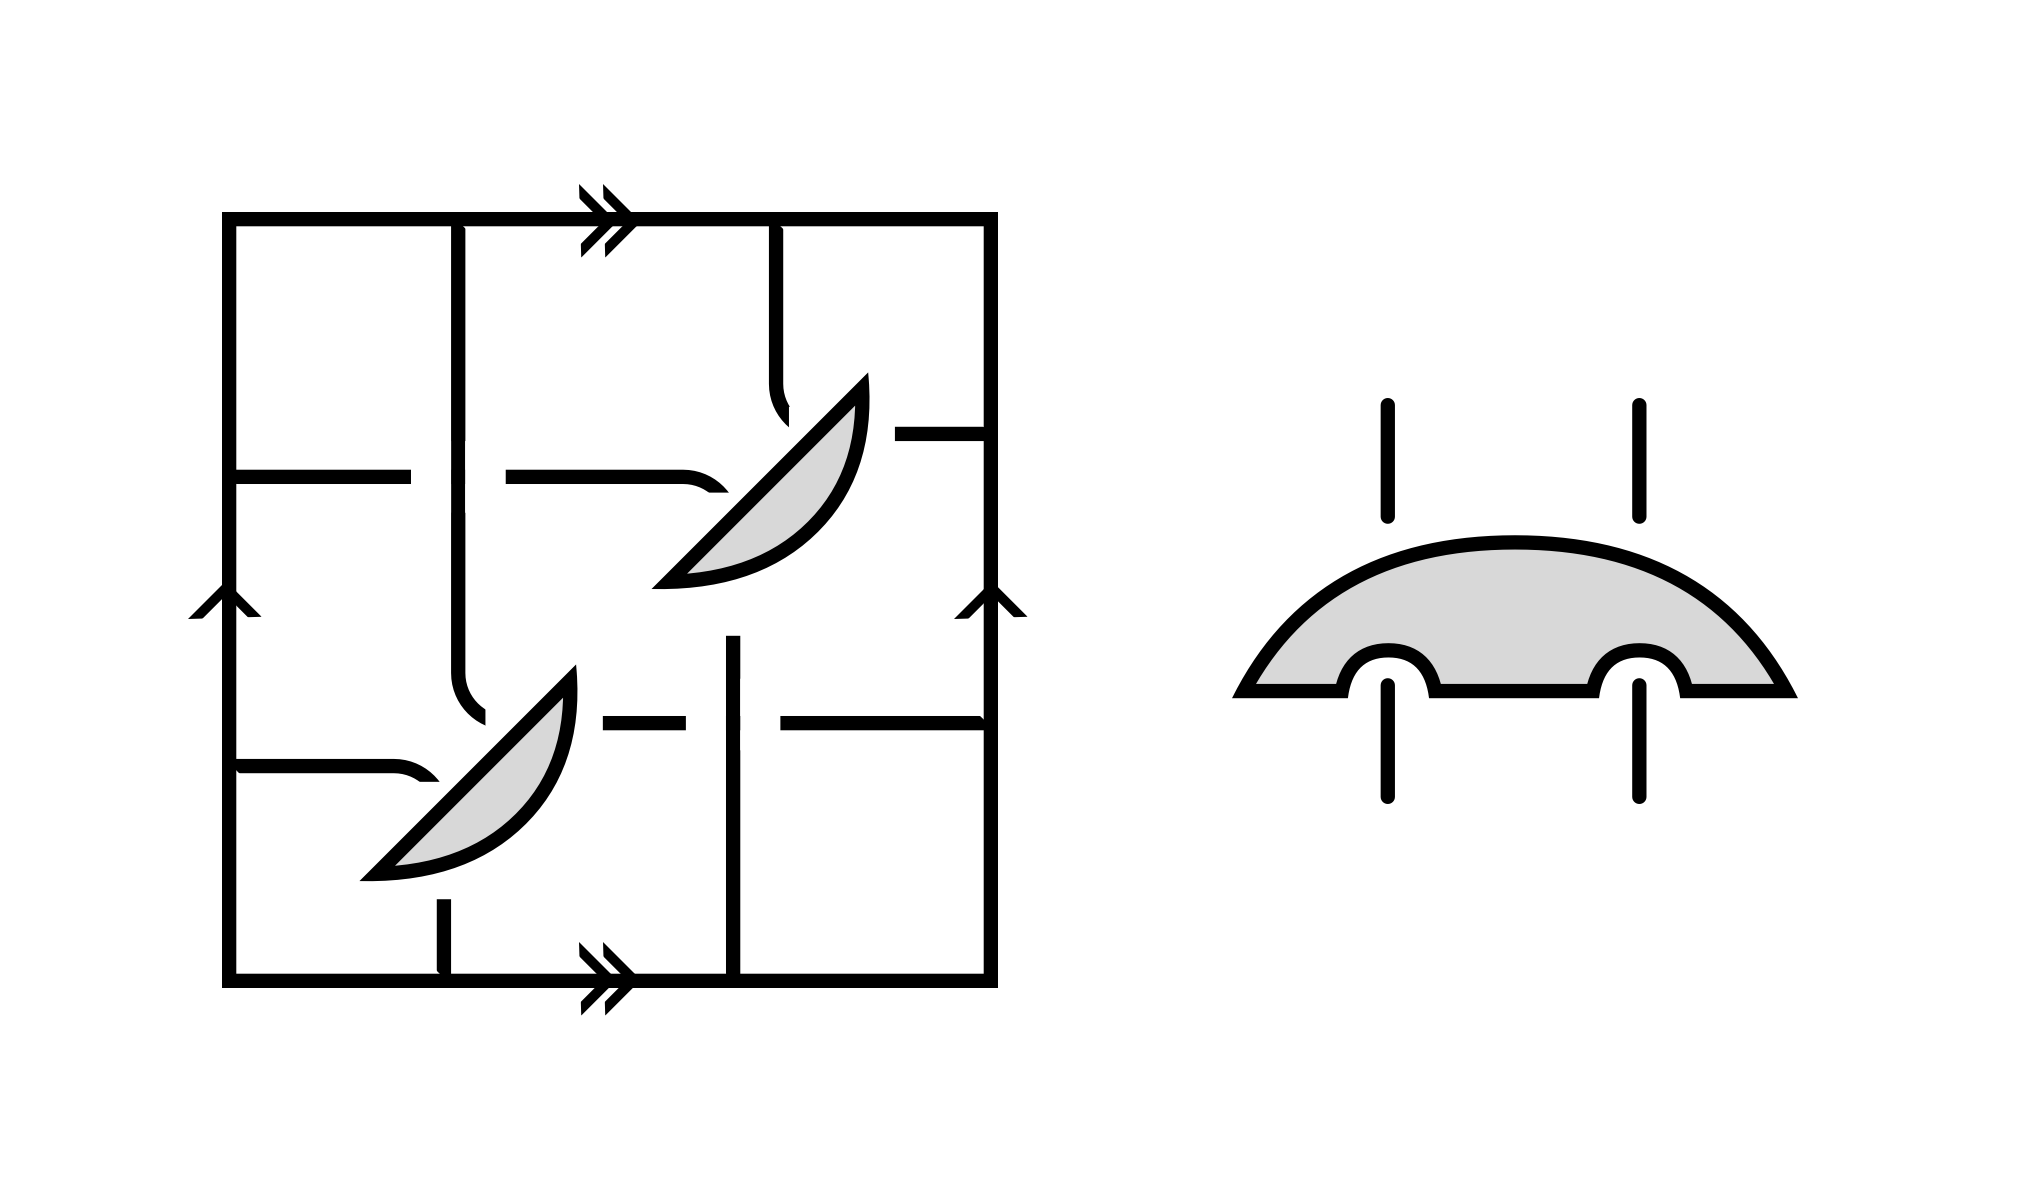
\includegraphics[height=3cm]{fig-4.png}
	\caption{Each crossing circle bounds a twice-punctured disk}
	\label{fig:step_one}
\end{figure}
 
%\vspace{-0.5cm} 
\begin{figure}[h] 
\centering 
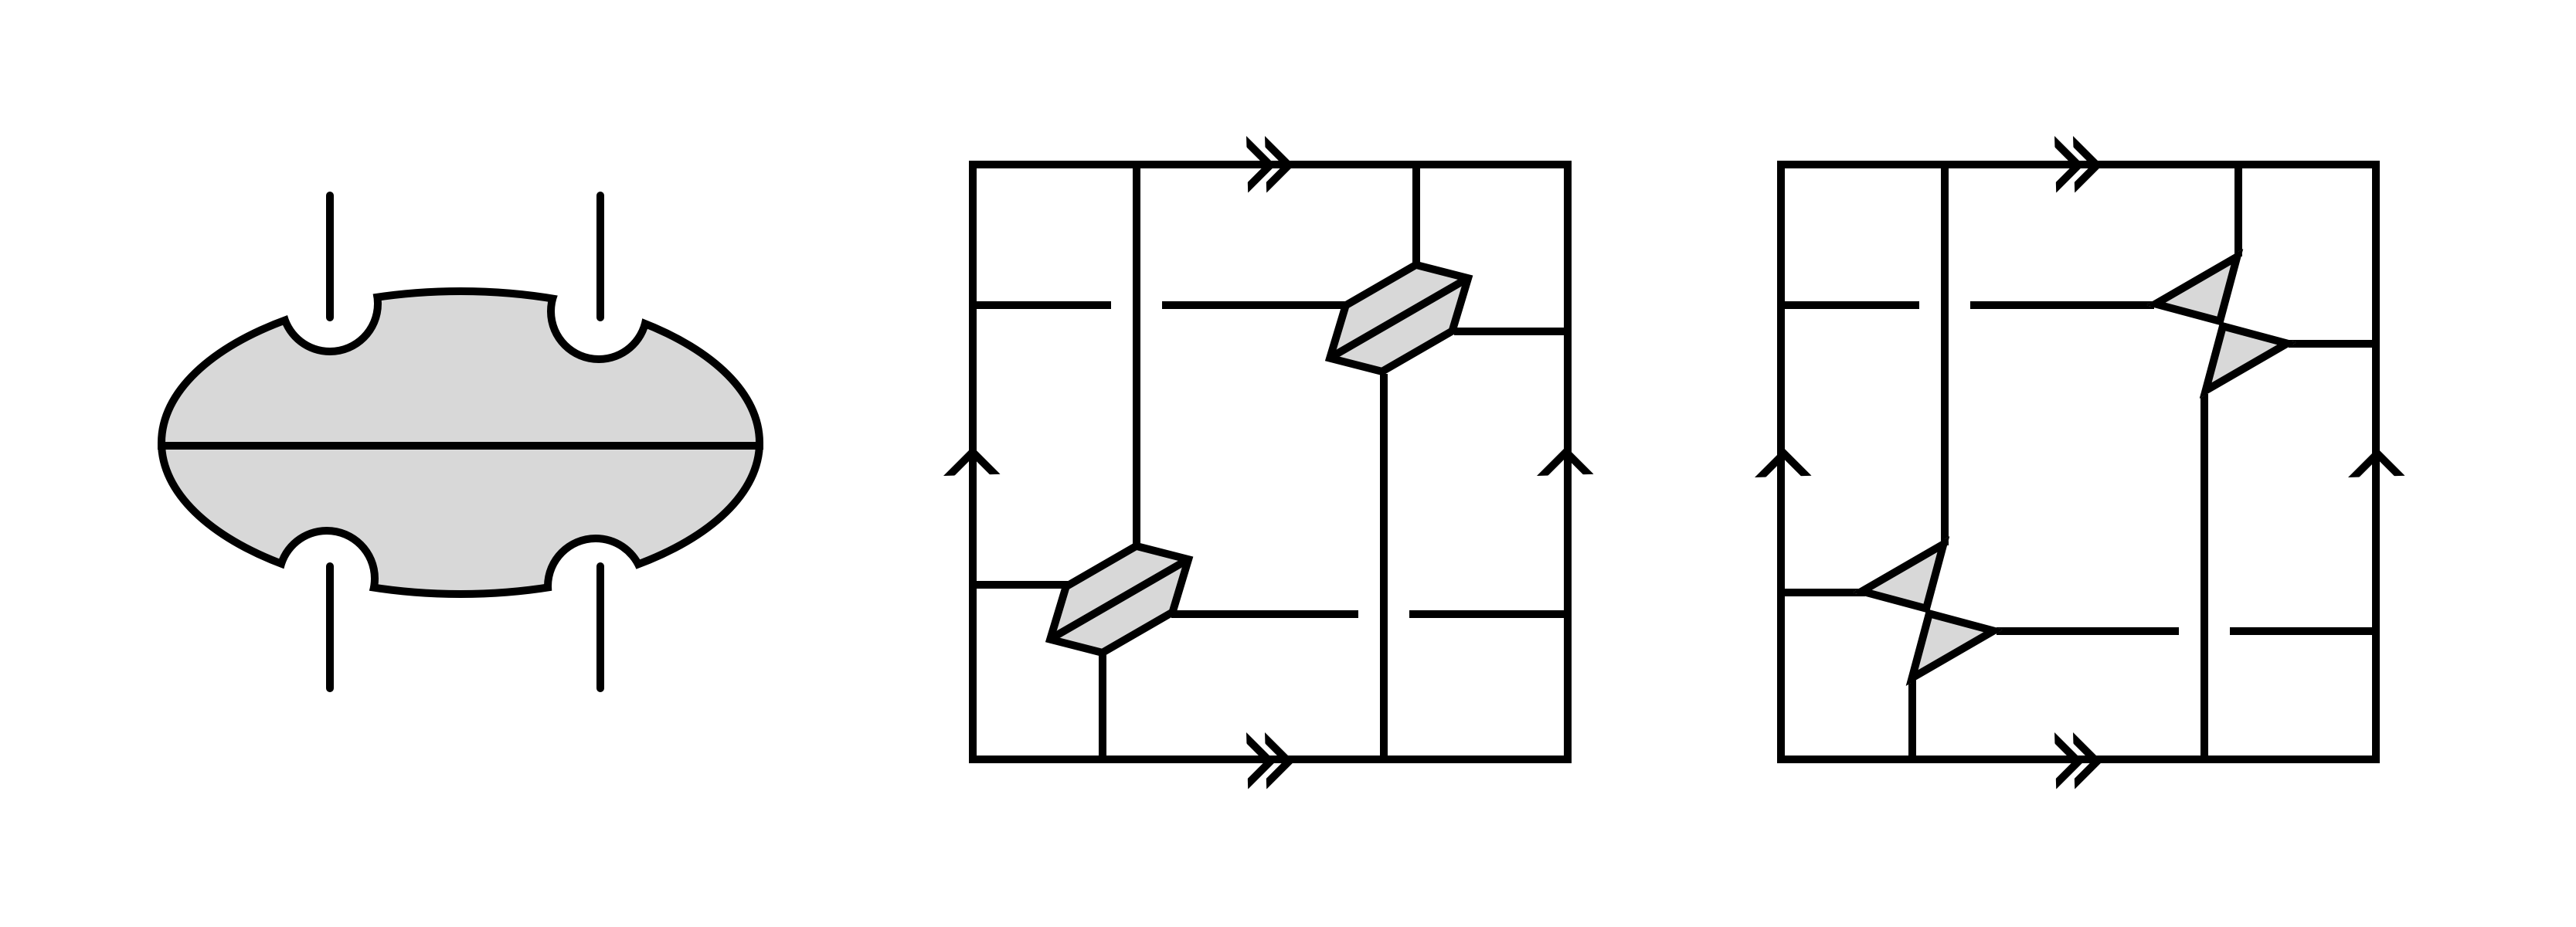
\includegraphics[height=3cm]{fig-5.png} 
	\caption{We split the disk and collapse the arc of each
 crossing circle to ideal vertices}
	\label{fig:step_two}
\end{figure}


\begin{figure}[h] 
\centering 
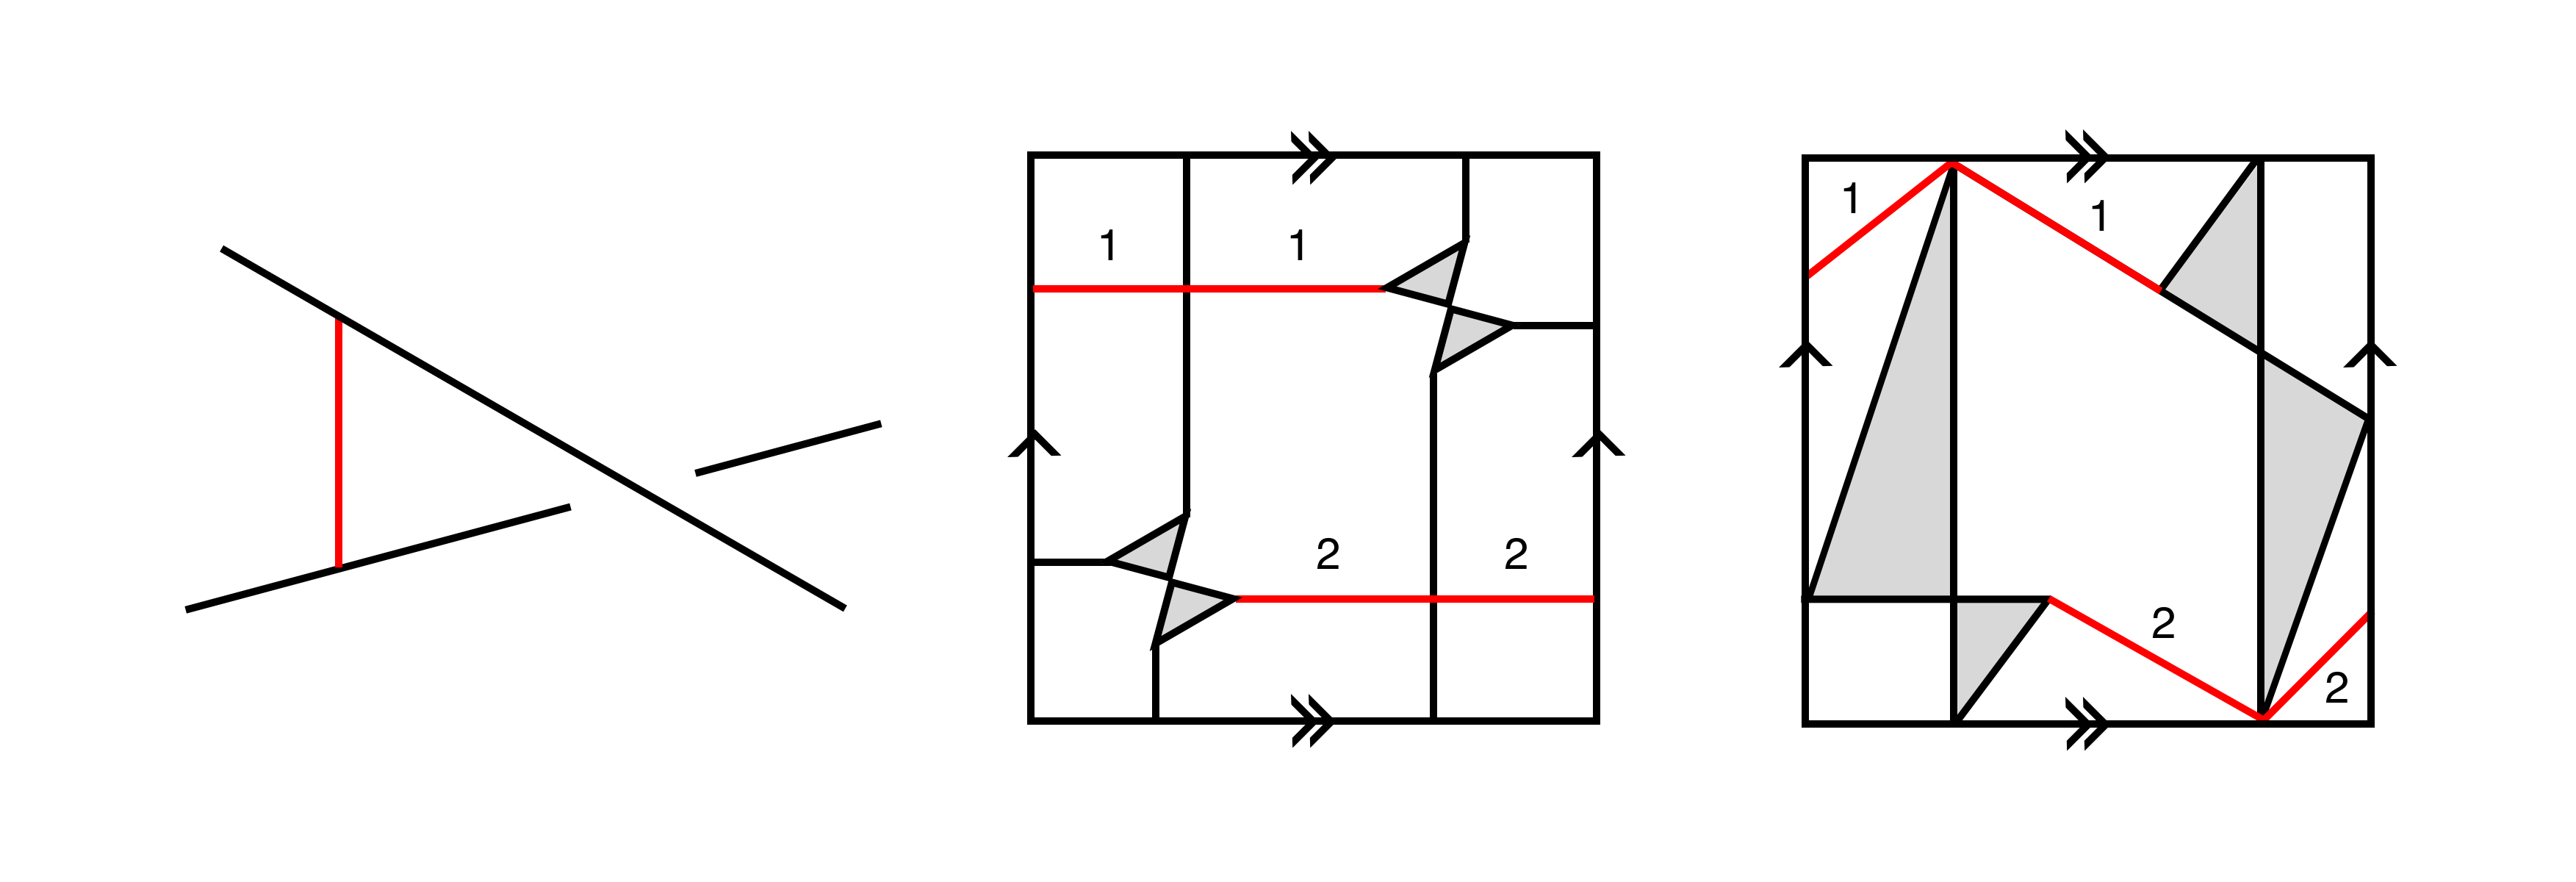
\includegraphics[height=3cm]{fig-6.png} 
\caption{Left: The crossing arc is the edge in red.
Middle: Picture of splitting the crossing edge. Right: The link component is
pushed off to infinity.}
	\label{fig:step_three}
\end{figure}

\begin{figure}[h] 
\centering 
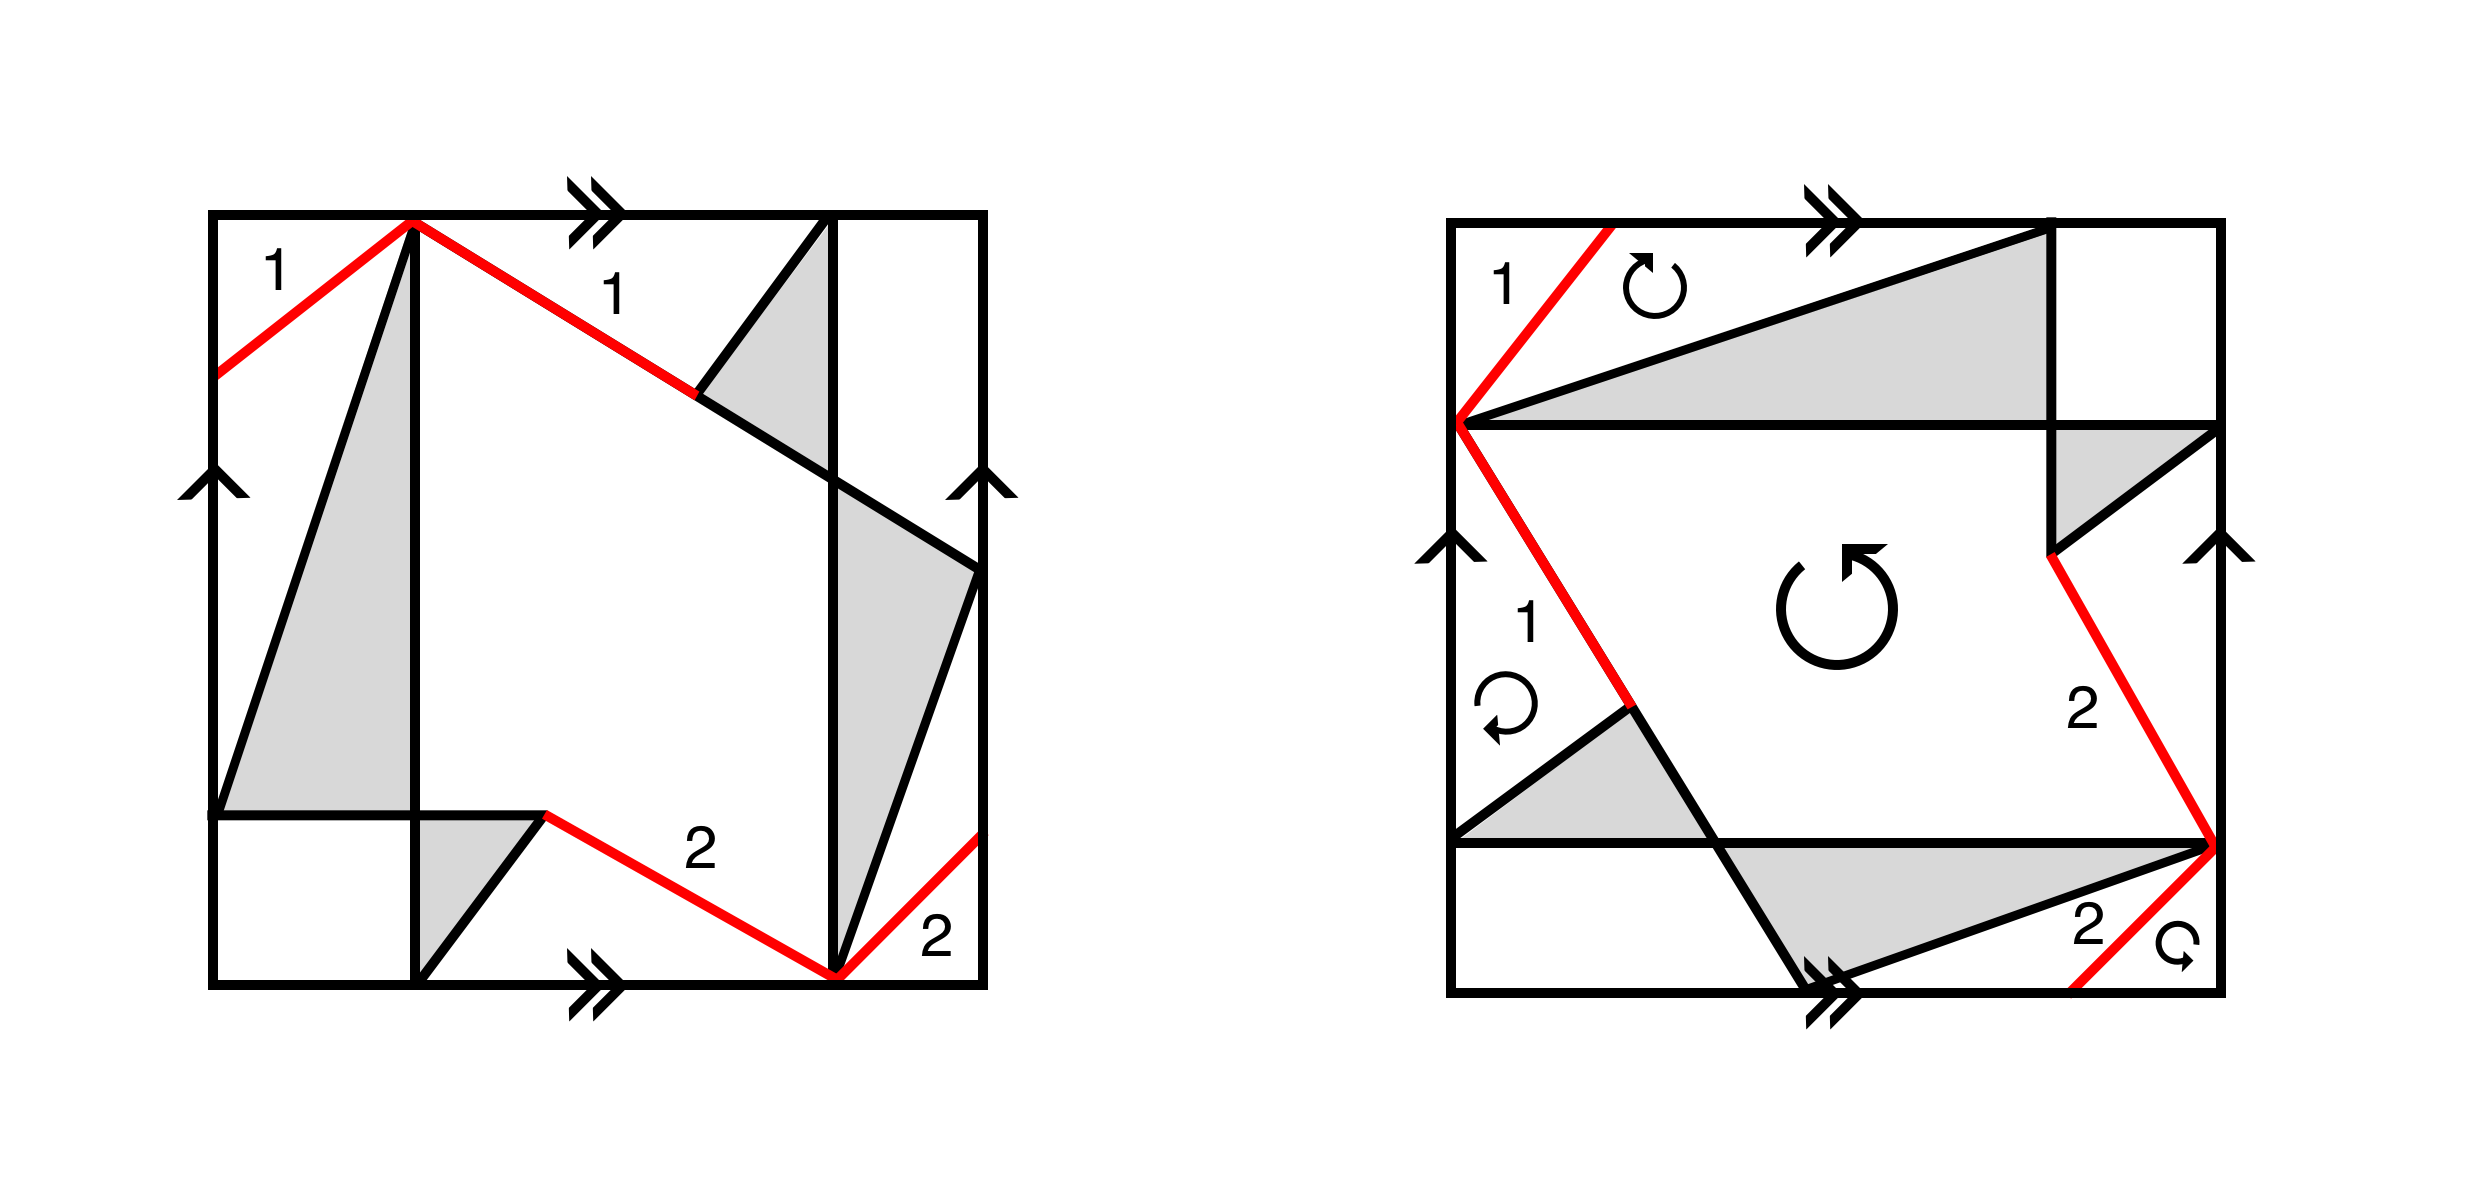
\includegraphics[height=3cm]{top-bottom.png} 
	\caption{Left: The top torihedron. Right: The bottom torihdron with rotation for face gluing.} 
\label{fig:top-bottom}
\end{figure}



\begin{definition}
An \emph{angled torihedron} $(\sT, \theta_\bullet^*)$
is a torihedron $\sT$ with
an assignment $\theta_e^* \in [0,\pi]$
such that for each vertex $v \in G(\sT)$,
$\sum_{e \ni v} \theta_e^* = (\deg(v) - 2)\pi$.
We also denote $\theta_e = \pi - \theta_e^*$,
so $\sum_{e \ni v} \theta_e = 2\pi$;
we refer to $\theta_e$ as the exterior angle
and $\theta_e^*$ as the interior angle. 
For brevity, we write dihedral angle to mean 
interior dihedral angle.  


We say $(\sT, \theta_\bullet^*)$ is \emph{degenerate}
if $\theta_e^* = 0$ for some edge;
we say it is \emph{non-degenerate} otherwise.
\end{definition}


One may ask for the pyramidal decomposition of a torihedron
to ``respect" angles. The following definitions,
in particular an ``angle splitting'', make sense of this.

\begin{define}
An \emph{angled ideal tetrahedron} is an ideal tetrahedron with an assignment of an
dihedral angle to each edge, such that
\begin{itemize}
\item each dihedral angle is in $[0, \pi]$;
\item for each tetrahedron, opposite edges have equal dihedral angles;
\item the three distinct interior angles at edges incident to one vertex sum to $\pi$.
\end{itemize}

We say an angled ideal tetrahedron is \emph{degenerate} if
one dihedral angle is 0; we say it is \emph{non-degenerate} otherwise.
\end{define}


\begin{define}
A \emph{base-angled ideal pyramid}
is a pyramid whose base is an $n$-gon, $n \geq 3$,
and each boundary edge $e_i$ of the base face is assigned a dihedral angle
$\alpha_i \geq 0$ such that the sum is $\sum \alpha_i = 2\pi$.
The vertical edge $e_i'$ that meets $e_i$ and $e_{i+1}$
is automatically assigned the dihedral angle $\pi - \alpha_i - \alpha_{i+1}$.


We say a base-angled ideal pyramid is \emph{degenerate} if
$\alpha_i = 0$ for some $i$; we say it is \emph{non-degenerate} otherwise.
\end{define}


Clearly, the dihedral angles of an ideal hyperbolic pyramid
make it a base-angled ideal pyramid
(with $\alpha_i = \vphi_{e_i}$);
it is not hard to see that the converse is true:
simply consider a circumsribed polygon such that the side $e_i$
subtends an angle of $2\alpha_i$ at the center,
and take the ideal hyperbolic pyramid over it in upper-half space.
Also, an angled ideal tetrahedron is simply a base-angled ideal pyramid
with base a triangle, and with no preferred face.

\begin{definition}
%TODO: this definition should come after base-angled pyramid
An \emph{angle splitting} of an angled torihedron $(\sT,\theta_\bullet^*)$
is a splitting of $\theta_e^* = \vphi_{\vec{e}} + \vphi_{\cev{e}}$
for each edge $e$,
such that for each face $f$,
$\sum_{\vec{e} \in \del f} \vphi_{\vec{e}} = \pi$.

Equivalently, an angle splitting is a decomposition of
$\sT$ into base-angled pyramids,
one for each face of $G(\sT)$, such that
for each boundary edge $e$ of $\sT$,
the dihedral angles from the two adjacent pyramids
add to $\theta_e^*$.
\end{definition}

\begin{remark}
These $\theta$'s are related to the $\theta$'s in
\cite{BandS},
and the $\vphi$'s are related to their ``coherent angle system''.
\end{remark}


%TODO remark on what splitting means in terms of ideal hyperbolic

\begin{lemma}
\label{l:pyramid_decomp}
%Let $P_n$ be an ideal pyramid whose base is an $n$-gon and suppose,
%\begin{itemize}
%\item each boundary edge of the base face is assigned a dihedral angle $\alpha_i$ such that for adjacent edges, $\alpha_i + \alpha_{i+1} < \pi$;
%\item we are given a decomposition of the base face into triangles by adding new edges. 
%\end{itemize}
Let $P_n$ be a base-angled ideal pyramid, and suppose we are given a
decomposition of the base face into triangles by adding new edges.  One gets an
obvious corresponding triangulation of $P_n$, where a new face is added for each
new edge. Then there is an assignment of a dihedral angle to each edge of each
ideal tetrahedron in this triangulation such that
\begin{itemize}
\item each tetrahedron is an angled ideal tetrahedron;
\item the sum of dihedral angles around each new edge is $\pi$;
\item the dihedral angles of the edges of the original base face are the same as
	before.
\end{itemize} 
\end{lemma}

\begin{proof}
Induct on $n$; there is nothing to prove for the base case $n=3$.

The proof is essentially given in Figure \ref{f:ideal_pyramid_arg}.

\begin{figure}
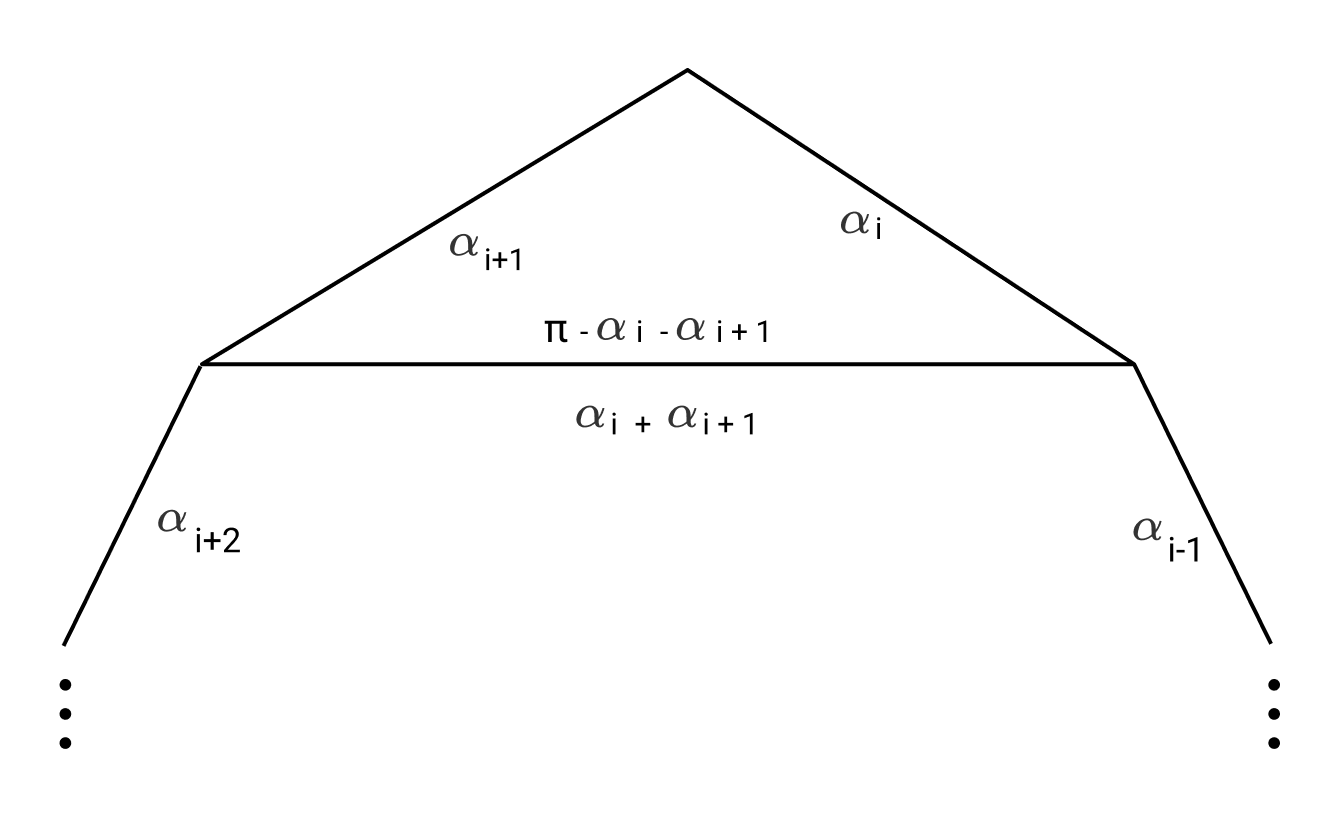
\includegraphics[height=5cm]{more_pictures/angle_split.png}
\caption{Angle-splitting on a polygonal face of the graph}
\label{f:ideal_pyramid_arg}
\end{figure}


Suppose the edges are labeled $e_i$, for an edge
which goes between vertices $v_i$ and $v_{i+1}$,
and suppose $e_i$ is assigned dihedral angle $\alpha_i$.
Let $e'$ be a new edge addeed to the base face of $P_n$
such that it separates the base face into a triangle and
an $(n-1)$-gon;
suppose the sides of the triangle are
$e_i, e_{i+1}$, and $e'$.
The new face corresponding to $e'$ separates $P_n$ into
an ideal tetrahedron $T$ and an ideal pyramid $P_{n-1}$.
We assign the dihedral angle of $\pi - \alpha_i - \alpha_{i+1}$
to $e'$ in $T$, and assign $\alpha_i + \alpha_{i+1}$ to $e'$ in $P_{n-1}$.
Clearly the sum of dihedral angles condition is satisfied
in $T$ and $P_{n-1}$.
It remains to check that the dihedral angles assigned to the vertical (non-base)
edges are correct.
For the vertical edge associated to $v_j$ for $j \neq i, i+2$,
there is nothing to check;
for $j = i$, the dihedral angles are
$\pi - \alpha_i - (\pi - \alpha_i - \alpha_{i-1})$
in $T$ and $\pi - \alpha_{i-1} - (\alpha_i + \alpha_{i+1})$ in $P_{n-1}$,
which sum to $\pi - \alpha_i - \alpha_{i+1}$;
it is similar for $j = i+2$.

\end{proof}




%%%%%%%%%%%%%%%%%%%%%%%%%%%%%%%%%%%%%%%%%%%%%%%%%%%%%%%%%%%
\section{Hyperbolicity of Augmented Links}
\label{s:hyperbolicity}
Thurston introduced a method for finding the unique complete hyperbolic metric for a
given 3-manifold $M$ with boundary consisting of tori \cite{Thurston}. 
%The idea
%was to triangulate the interior of $M$ into ideal tetrahedra and give those
%tetrahedra hyperbolic shapes (called shape parameters) that glue up coherently
%in $M$. The shape parameter of a tetrahedron is described by the cross-ratio of
%its four vertices on the sphere at infinity. 
Thurston had written down a system
of gluing and consistency equations which can be translated to 
equations with angles for a triangulation of $M$ whose solutions correspond to the
complete hyperbolic metric on the interior of $M$. Casson and Rivin separated Thurston's
gluing equations into a linear and non-linear part \cite{Casson-Rivin}. Angle
structures is the linear part of Thurston's gluing equations, and what we will
use to attain hyperbolicity of complements of augmented links in the thickened
torus.


\begin{define}
Let $M$ be an orientable 3-manifold with boundary consisting of tori. An angle
structure on an ideal triangulation $\tau$ of $M$ is an assignment of a dihedral
angle to each edge of each tetrahedron, such that
\begin{itemize}
\item each tetrahedron is a non-degenerate angled ideal tetrahedron,
\item around each edge of $\tau$, the dihedral angles sum to $2\pi$.
\end{itemize}
\end{define}

\begin{theorem}\cite{TODO: find rivin's paper? should be in here https://arxiv.org/pdf/1004.0440.pdf}
Let $M$ be a 3-manifold admitting an angle structure. Then $M$ is hyperbolic.
\end{theorem}

For a hyperbolic link $K$ in $\torus \times I$, we show
that the resulting link obtained from augmenting $K$ is
hyperbolic. The idea is to start with a graph from the torihedral decomposition
of the link $K$ which will give us a graph on each torihedron with an angle
assignment of
$\pi/2$ for edge
\cite{CKP2}.
By \prpref{p:tori_decomp},
there is a torihedral decomposition of the complement of the augmented link $L$.
Using those angles from $K$,
we then assign new angles locally to edges of torihedra from a torihedral 
decomposition of $L$
and decompose them into base-angled pyramids which can be decomposed 
into tetrahedra, thus obtaining an angle structure on a triangulation.


\begin{define}
We say an augmentation is \emph{right-augmented} if, when both strands are
(locally) oriented so that they cross the augmentation disk in the same
direction, the crossing between them is a positive right-handed half-twist.
See Figure \ref{f:right_left_aug}.
We say an augmentation is \emph{left-augmented} if it is not right-augmented.
\end{define}

\begin{figure}
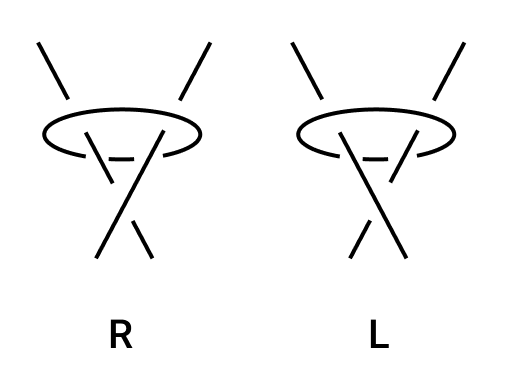
\includegraphics[width=5cm]{more_pictures/right_left_aug.png}
\caption{R: right augmentation, L: left augmentation}
\label{f:right_left_aug}
\end{figure}

We can recover $L$ from the link diagram of $K$
together with labels at vertices indicating left- or right-augmentation.


\begin{lemma}
\label{l:2fe}
Let $G$ be a 4-valent graph on $\torus$ with no bigons or self-loops.
%and whose faces can be checkerboard colored.
Then for any subset $F' \subseteq F$ of faces,
\[
	2\chi(F') \leq |E'|
\]
where $E' = \cup_{f \in F'} \del f$ is the set of edges
that meets some face of $F'$,
and $\chi(F') = \sum_{f\in F'} \chi(f)$ is the sum
of the Euler characteristics of faces in $F'$.
\end{lemma}

\begin{figure}
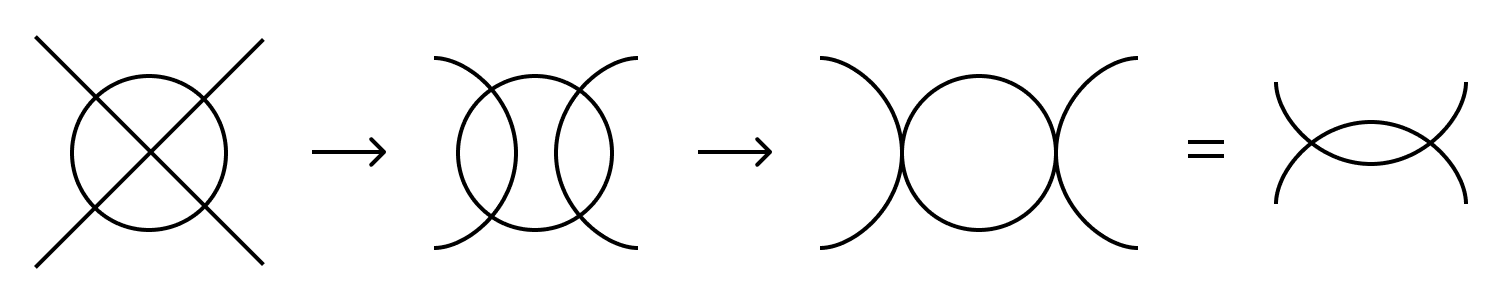
\includegraphics[width=11cm]{bigon_crush.png}
\caption{Resolving internal vertex; eliminating bigons via ``crushing"}
\label{f:bigon_crush}
\end{figure}

\begin{proof}
We induct on $\chi(F')$  (over all possible such graphs $G$);
for $F' = \emptyset$ or $\chi(F') \leq 0$, there is nothing to prove.

Call a vertex or edge \emph{interior} if it does not meet
$F'' = F \backslash F'$.
Suppose there is an interior vertex $v$.
Make the modification as in Figure \ref{f:bigon_crush}
(later we will choose which way to ``resolve'' the vertex).
This decreases $\chi(F')$ by one and $|E'|$ by 2.
However, this process may produce bigons;
if it does, repeatedly eliminate bigons by either
(1) performing the modification as in Figure \ref{f:bigon_crush}
if the two vertices of the bigon are distinct,
or (2) remove the bigon completely if the two vertices
of the bigon are the same.
Each of these steps also decreases $\chi(F')$ by one and $|E'|$ by 2
(note in the second case, after removing the bigon,
the operation merges two distinct faces or joins a face to itself;
this adds an $S^1$, thus does not change the (total) euler characteristic
of the two faces or the one face).


We must check that this process terminates with a graph
which satisfies the hypotheses set out in the lemma.
It is clear that %checkboard colorability and
4-valency is maintained
at each step, and there will not be any bigons at the end.
We need to ensure that eliminating bigons does not
create self-loop edges.
Here we specify how to choose which way to resolve the internal
vertex $v$. If among the four faces touching $v$,
one of them has greater than three sides (Case 1),
then resolve $v$ so that this face is not merged;
if all four faces are triangles (Case 2),
simply resolve in an arbitrary manner.
After the modification of the internal vertex,
at most two bigons are created;
eliminate those two bigons.
Now we find that all bigons will be connected end-to-end
(i.e. forming a single twist region) -
this is because in Case 1, only one bigon was present after smoothing
$v$, which would result in at most two bigons that would be connected;
and if we were in Case 2, we find that the face between those
eliminated bigons (coming from merging the two triangles across $v$)
will become a bigon too,
thus connecting the potential bigons on either ends.

Therefore, one can eliminate bigons in an order so that
they belong in one twist region;
in particular, the (not necessarily distinct) faces on either side
are not bigons,
so eliminating the bigon does not produce a self-loop edge.


Now suppose $G$ has no interior vertices.
We perform some reductions.
We remove all $f$ from $F'$ that have non-positive Euler characteristic,
as doing so will not decrease $\chi(F')$ and will not increase $|E'|$.
Now consider some $f\in F'$.
If it has at least two boundary (i.e. non-interior) edges,
we can remove $f$ from $F'$,
which decreases $\chi(F')$ by 1 and $|E'|$ by at least 2.
Thus we remove all such $f$.


Now suppose $f\in F'$ has three contiguous interior edges
$e_1,e_2,e_3$.
(e.g. if $f$ has at least four sides).
Let $v_1, v_2$ be the vertices between these three interior edges.
Since $v_1$ is not interior,
the face across $v_1$ from $f$ is not in $F'$;
likewise with $v_2$.
But this shows that the face across $e_2$ from $f$
has two boundary edges, contradicting our reduction.
%This would lead to the situation in \ref{},
%showing that there is a face with at least
%two boundary edges, contradicting our reduction.


Thus, we now have a graph whose faces are triangles,
and each face has exactly one boundary edge.
Now the problem is solved with a simple counting argument:
each $f$ corresponds to one boundary edge and two interior edges,
but, since the interior edges are shared by two faces,
they should count as half an edge; so
\[
 |E'| = \sum_{f\in F'} 1 + 1/2 + 1/2 = 2|F'| = 2\chi(F')
\]
and we get the desired result.
\end{proof}


The following theorem is quoted from \cite{BandS}
(see also \cite{FF})

\begin{theorem}[Feasible Flow Theorem]
\label{t:feasible_flow}
Let $(N,X)$ be a directed graph,
with a \emph{lower capacity bound} $a_x$
and \emph{upper capacity bound} $b_x$
for each directed edge $x \in X$,
with $-\infty \leq a_x \leq b_x \leq \infty$.
A \emph{feasible flow} is a function $\vphi : X \to \RR$
such that $\vphi_x \in [a_x, b_x]$ and
Kirchhof's current law is satisfied
(i.e. flow in = flow out at every vertex).

A feasible flow exists if and only if,
for every proper nonempty subset $N' \subset N$,
\[
\sum_{x \in ex(N')} b_x \geq \sum_{x \in in(N')} a_x
\]
where $ex(N'), in(N')$ refer to edges leaving,
entering $N'$, respectively.
\end{theorem}



\begin{theorem}
\label{t:auglink_hyp}
Let $K$ be a weakly prime, alternating link whose diagram has no bigons.
Let $L$ be a link obtained from augmenting $K$.
Then $L$ is hyperbolic.
\end{theorem}

\begin{proof}
By \cite[Theorem 7.5]{CKP2},
(as discussed in \prpref{p:tori_decomp},)
$\toruscomp{K}$ can be decomposed
into two torihedra $\sT_T$ and $\sT_B$,
whose graphs are $\Gamma_T(K), \Gamma_B(K)$ respectively;
viewed from the top cone point $\torus \times \{1\}$,
they are both the same as the projection graph of $K$.
%which we denote by $\Gamma$.
We make them non-degenerate angled torihedra by assigning $\theta^* = \pi/2$
for all edges. Unlike in the case of alternating links or fully augmented links 
in the thickened torus we cannot make all angles $\pi/2$. This is 
because in our decomposition the vertices of the graph which
defines our torihedra are not all four valent. 

We obtain an angle-splitting by applying the
Feasible Flow theorem (\thmref{t:feasible_flow}) as follows:
Consider the directed graph whose vertex set is
$E \cup F \cup \{*\}$,
where $E, F$ are the set of edges, faces of $\Gamma_T(K)$ respectively,
%and $*$ is some abstract vertex.
and there is a directed edge
\begin{itemize}
\item $* \to f$ for each face $f\in F$, with capacity interval
	$[\pi, \infty)$,
\item $f \to e$ for each edge $e \in \del f$,
	with capacity interval $[\veps, \infty)$
	for some $\veps>0$ to be set later,
\item $e \to *$ for each edge $e$, with capacity interval
	$(-\infty, \pi/2]$.
\end{itemize}
By \lemref{l:2fe}, $2|F'| = 2\chi(F') \leq |E'|$,
and taking $\veps < \pi / |\text{max face size}|$,
the feasible flow condition is satisfied,
so a feasible flow exists.
Since $2|F| = |E|$, the capacity interval restrictions
on the flow at $*$ is sharp, so out-edges at $*$
have flow $\pi$ and in-edges at $*$ have flow $\pi/2$.
Then the flow $f \to e$ gives us $\vphi_{\vec{e}}$,
where $f$ is the face to the left of $\vec{e}$.
(We adapted this argument from Lemma 3.4 of \cite{BandS}).


\begin{figure}
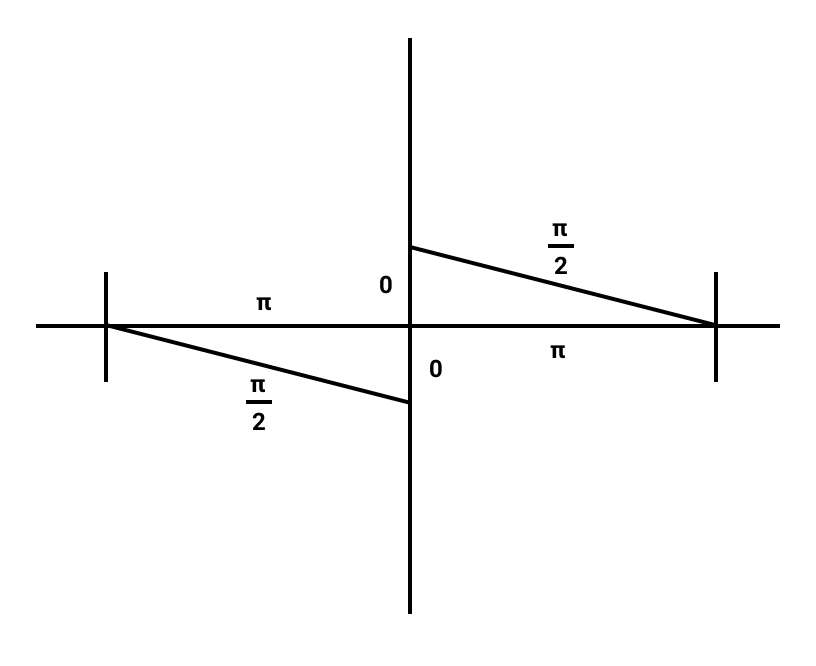
\includegraphics[width=7cm]{more_pictures/horizontal_bowtie.png}
\caption{Angle assignments on a bow-tie corresponding to an augmentation site}
\label{f:bowtie_angles}
\end{figure}

By \prpref{p:tori_decomp}, $\toruscomp{L}$ can be
obtained by gluing two torihedra $\sT_T(L),\sT_B(L)$
with graphs $\Gamma_T(L),\Gamma_B(L)$.
We make them degenerate angled torihedra by assigning $\theta^*$'s
to edges of the bow-ties as in Figure \ref{f:bowtie_angles},
and assign $\pi/2$ to all other edges.
It is easy to check that upon gluing,
each edge has sum of dihedral angles ($\theta^*$) that is equal to $2\pi$.
(This holds true even if they were glued assuming
some augmentations had no half-twist; see \remref{r:nohalftwist}.)


Furthermore, we can obtain an angle-splitting of $\sT_T(L)$
(and similarly $\sT_B(L)$) by modifying the angle-splitting
for $\sT_T(K)$;
this is shown in Figure \ref{f:bowtie_angles2}. 


\begin{figure}
\begin{tabular}{cc}
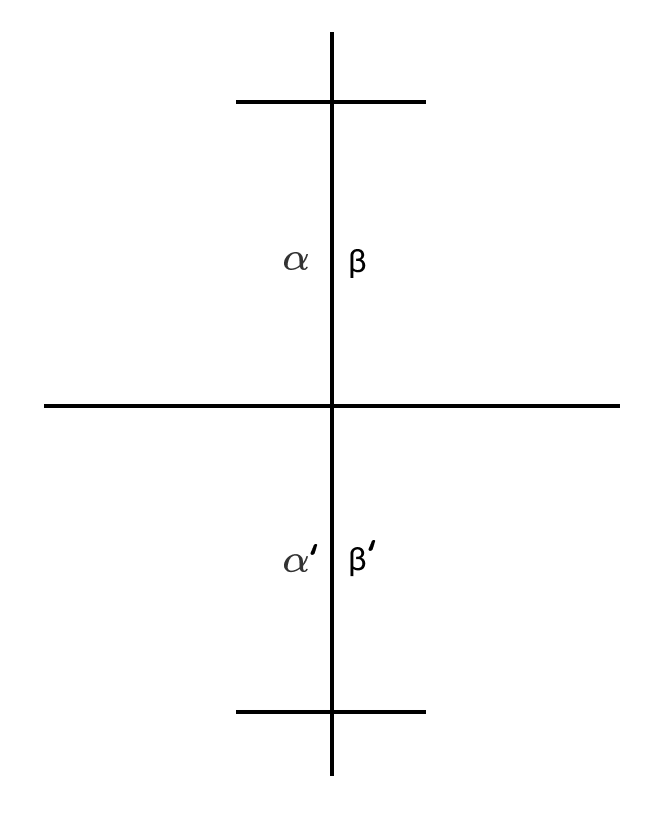
\includegraphics[width = 5cm]{before_bowtie_angles.png}&
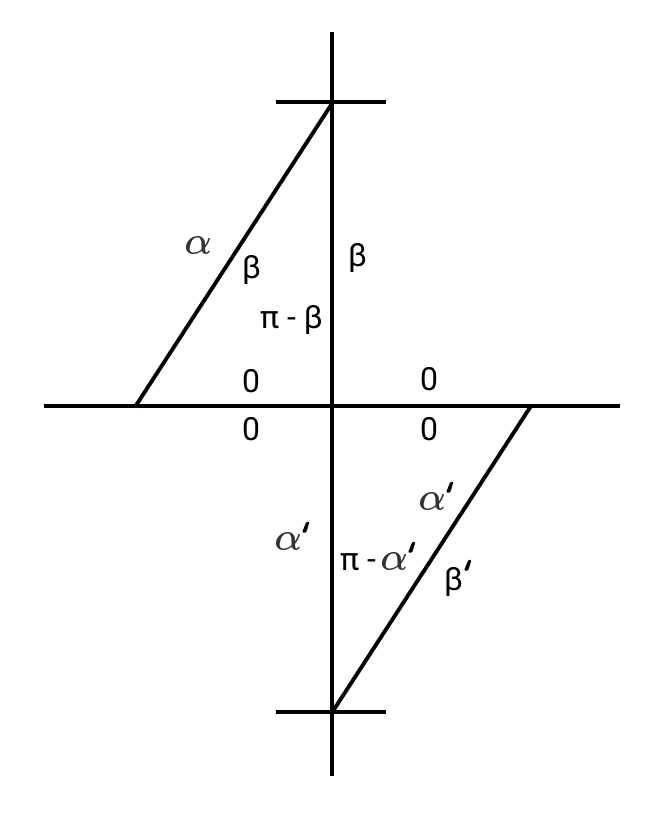
\includegraphics[width = 5cm]{bowtie_angles.png}\\
(a)&(b)
\end{tabular}
\caption{(a) Angles before augmentation (b) Angle splitting for bowtie corresponding to augmentation}
\label{f:bowtie_angles2}
\end{figure}

Now we have a decomposition of the two torihedra into
degenerate base-angled pyramids.
However, we need the pyramids to be non-degenerate,
so we first need to modify the angles and graph on the torihedra
to make all $\theta^*$ nonzero.


Consider a face $f$ of $\Gamma_T(L)$ that is not in a bow-tie.
Suppose the corresponding face $\bar{f}$ of $\Gamma$,
the projection graph (which is equal to $\Gamma_T(K)$),
had vertices $v_1,\ldots,v_n$ in counter-clockwise order.
We label the edges of $f$ by $e_{i,0}$, $e_{i,\pi}$, or $e_i$,
depending on whether the $\theta^*$ is $0$, $\pi$, or $\pi/2$ respectively,
with $i$ non-decreasing from 1 to $n$,
adjacent edges having the same $i$ if and only if they
belong to the same bow-tie.
For sake of concreteness,
suppose that if a vertex $v_i$ is right-augmented,
then the augmentation circle intersects $\bar{f}$
(everything is similar if it is left-augmented vertices' circles
that intersect $\bar{f}$).
In other words, locally, $f$ meets two of the edges of the bow-tie
corresponding to a right-augmented vertex $v_i$
(which would be labeled $e_{i,0}, e_{i,\pi}$ in counter-clockwise order),
but only meets one of the edges of the bow-tie corresponding to
a left-augmented vertex.


Suppose, after cyclically reindexing, $v_1,\ldots,v_k$
is a maximally contiguous subsequence of left-augmented vertices
of $G(K)$ around the face $\bar{f}$;
the edges around $f$ would start
$e_{1,0}, e_{1,\pi}, e_{2,0}, e_{2,\pi}, \ldots$.
We add new edges across $f$ as follows.
(See Figure \ref{f:adding_edges};
ignore the + and - signs for now.)


First suppose $k=n$; then we do nothing.

Next suppose there is only one such maximal contiguous subsequence.
If $k = 1$, we add an edge that goes across
$e_{1,0},e_{1,\pi},e_2$
(in the sense that the new edge separates the edges of $f$ into two sets,
one of them being those three edges;
since $n\geq 3$, this edge is new).
%If $k = 2$, we add edge across $e_{1,0},e_{1,\pi}$
%and another edge across $e_{2,0},e_{2,\pi}$
%(these two edges do not form a bigon because we've ruled out $k=n$).
%(these two edges do not form a bigon because we've ruled out $k=n$).
If $k \geq 2$,
we add an edge across $e_{1,0},e_{1,\pi}$
and another edge across $e_{2,0},e_{2,\pi},e_{3,0},\ldots,e_{k,\pi}$
(these two edges do not form a bigon because we've ruled out $k=n$).
%(again these two edges do not form a bigon).

Finally, if there are multiple such maximal contiguous subsequences,
we just add edges as above for each contiguous subsequence.
The only caveat is that if the procedure calls to add a new edge
that would form a bigon with the existing edges,
we just do not add it.


This way we obtain a new graph $\Gamma_T(L)'$, which defines a
new torihedron $\sT_T(L)'$.
We make $\sT_T(L)'$ angled using the angles from $\sT_T(L)$ for old edges,
and putting $\pi$ for all new edges.


\begin{figure}
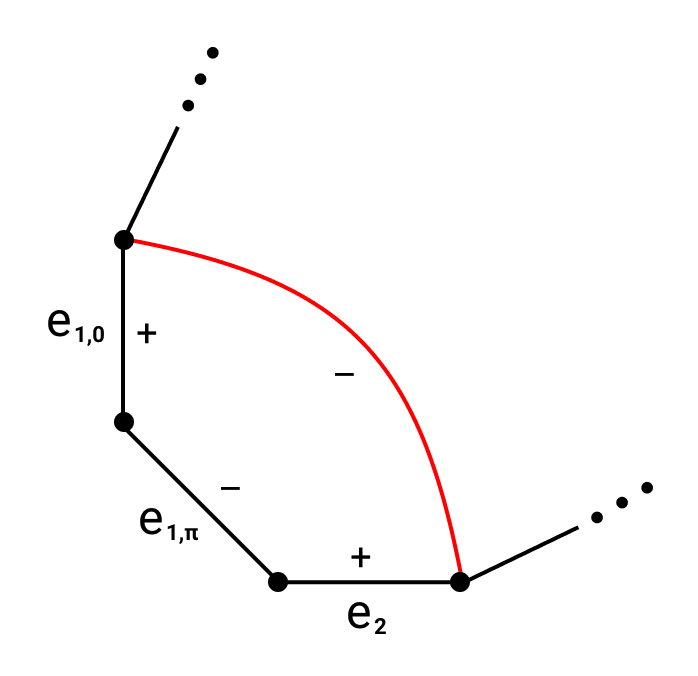
\includegraphics[width=5cm]{more_pictures/one_edge.png}
%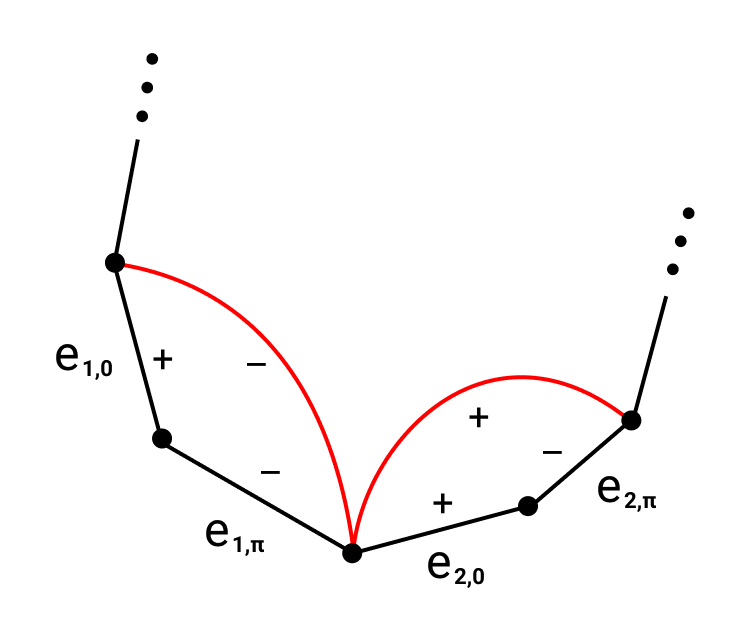
\includegraphics[width=5cm]{more_pictures/two_edge.png}
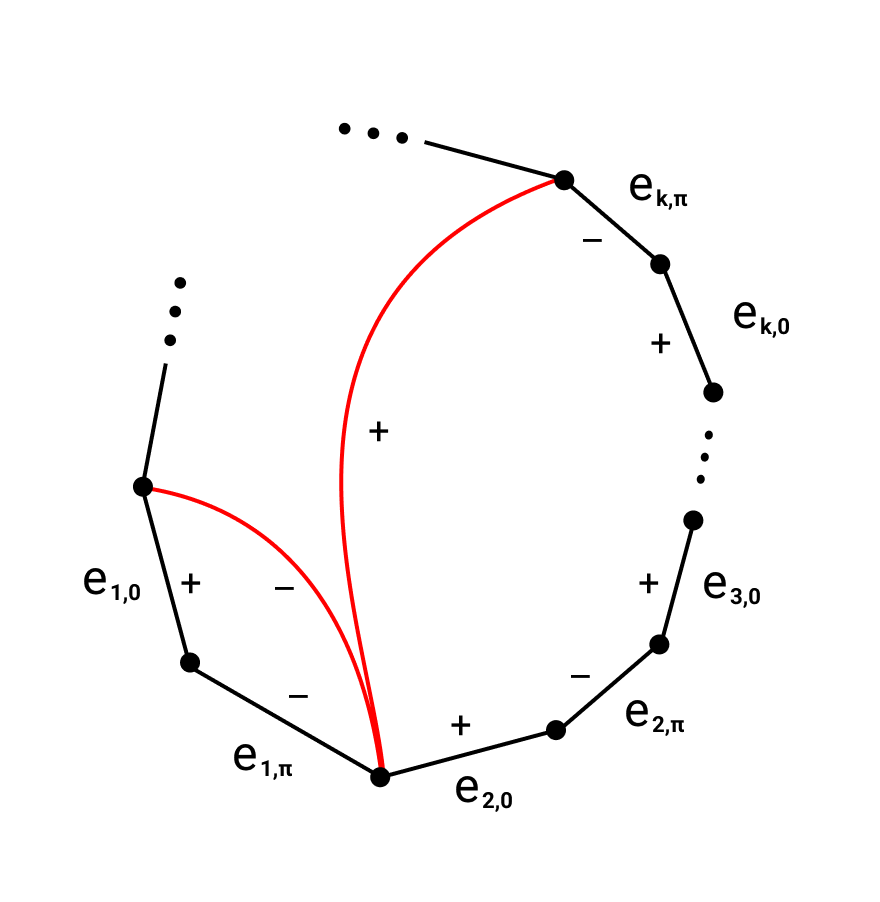
\includegraphics[width=5cm]{more_pictures/two_edge_many.png}
\caption{Red edge indicates an added edge to the graph to appropriately assign +/- labels which indicate 
increasing/decreasing angles on the edge respectively.}
\label{f:adding_edges}
\end{figure}

Now we deform the $\theta^*$ based on Figure \ref{f:adding_edges},
increasing/decreasing by some small $\veps' > 0$ if the edge
is labeled $+/-$.
Note some edges may be labeled twice, in which case we perform
both increasing/decreasing (e.g. if it is labeled $+$ and $-$,
the $\theta^*$ is not changed).
It is easy to see that the sum of $\theta^*$ around a vertex
remains unchanged.
Furthermore, all the edges with $\theta^*$ originally equal 0,
i.e. all $e_{i,0}$'s,
now have positive $\theta^*$,
(it receives only one label $+$,
because the other face it meets is a bow-tie).



%Thus, we could attempt to apply the feasible flow theorem in a similar manner,
%and obtain an angle-splitting for $\sT_T(L)'$, but 
%TODO rephrase nicely.
We can directly get an angle-splitting for $\sT_T(L)'$
using the angle-splitting for $\sT_T(L)$.
We reuse the $+/-$ assignments from Figure \ref{f:adding_edges}.
For $e = e_{i,0}$, we increase $\vphi_{\vec{e}}, \vphi_{\cev{e}}$
by $\veps'/2$ each; for $e = e_{i,\pi}$,
we decrease them by $\veps'/2$ each.
For other edges, we increase/decrease $\vphi_{\vec{e}}$ by $\veps'$,
where $\vec{e}$ is the oriented edge corresponding to the side
on which the $+/-$ sign appears in Figure \ref{f:adding_edges};
so for example, if an edge $e$ receives both $+$ and $-$,
then one of $\vphi_{\vec{e}},\vphi_{\cev{e}}$ increases
while the other decreases, thus $\theta_e^*$ remains constant.


Now we address $\sT_B(L)$.
In the gluing of $\sT_T(L)$ to $\sT_B(L)$,
non-bow-tie faces of $\Gamma_T(L)$ are identified with
non-bow-tie faces of $\Gamma_B(L)$.
Under this identification, we add the same edges to $\Gamma_B(L)$,
thus obtaining the new torihedron $\sT_B(L)'$ with graph
$\Gamma_B(L)'$.
We perform the same deformations of $\theta^*$'s (or $\vphi$'s).


We need to check that upon gluing $\sT_T(L)'$ to $\sT_B(L)'$,
the sum of dihedral angles around each edge is still $2\pi$.
This was clearly true before deforming, as the new edges of
$\Gamma_T(L)'$ only gets identified with the unique
corresponding edge of $\Gamma_B(L)'$, and they are both labeled
with $\theta^* = \pi$.
To see that the deformation does not change these sums,
note that in the identification of faces of $\Gamma_T(L)'$
to $\Gamma_B(L)'$,
an edge with $\theta^*=0$ is identified with an edge with
$\theta^*=\pi$,
so an increase in the former would be conterbalanced by
a decrease in the latter.
It is also easy to see this is the case for the other edges.
(Once again, a similar argument applies if $\sT_(L)'$
and $\sT_B(L)'$ are glued assuming
some augmentations had no half-twist; see \remref{r:nohalftwist}.)


Finally, for each face of $\Gamma_T(L)'$ that has more than three sides,
we arbitrarily decompose it into triangles
and apply \lemref{l:pyramid_decomp}
to obtain a triangulation of $\sT_T(L)'$ into non-degenerate angled tetrahedra;
perform the corresponding decomposition for faces of
$\Gamma_B(L)'$ and obtain a triangulation of $\sT_B(L)'$
into non-degenerate angled tetrahedra.
Upon gluing, this gives an angle structure on the triangulation
of $\toruscomp{L}$
\end{proof}



\begin{remark}
\label{r:nohalftwist}
If the original link $K$ had some twist regions with at least one bigon,
we may consider augmentations $L$ where all such twist regions
are augmented, i.e. $L$ may have augmentations without half-twists.
Then, as pointed out in proof of \thmref{t:auglink_hyp} above,
the proof still works for $L$, showing that $L$ is also hyperbolic.
\end{remark}



\bibliographystyle{plain}
\bibliography{references-ak}


\end{document}
